\documentclass[Letter,11pt]{book}

% QCC book needs
\usepackage{fix-cm}  % this package allows large \fontsize
\usepackage{imakeidx}
\makeindex[title=Index]
\usepackage{listings}
\usepackage[table]{xcolor}

\usepackage{amsmath,graphicx}

\usepackage{tikz}    % this is for graphics. e.g. rectangle on title 
\usetikzlibrary{quantikz, decorations.pathmorphing,shapes.geometric}
%\usepackage{circuitikz}
\usepackage{tikz-3dplot} % includes tikz
\tdplotsetmaincoords{70}{120}
\usepackage{float}


% This file is for commands / macros / functions.
% QCC book specific
\newcommand{\keta}[2][]{\vert {#2} \rangle_{#1}}
\newcommand{\braketa}[3][]{\langle {#2} \vert {#3}\rangle_{#1}}

\tikzstyle{Gate}=[rectangle, minimum width=30, minimum height=30, text width=20, text centered, draw=black]
% Content Starts Here
\begin{document}

%\title{Quantum Information, Algorithms and Protocols}
\author{Yuan John Jiang}

\newcommand{\booksubtitle}{A Textbook for Computer Science and Engineering Students}
\newcommand{\booklicense}{Creative Commons Zero 1.0 Universal}

% Author subtitle could be a university or a geographical location, for example
\newcommand{\authorsubtitle}{City, Country}

% Create convenient commands \booktitle and \bookauthor
\makeatletter
\newcommand{\booktitle}{\@title}
\newcommand{\bookauthor}{\@author}
\makeatother

% The following dimensions specify 4.75" X 7.5" content on 6 3/8" by 9 1/4"
% paper. The paper width and height can be tweaked as required and the content
% should size to fit within the margins accordingly.
%
% The (inside) bindingoffset should be larger for books with more pages. Some
% standard recommended sizes are .375in minimum up to 1in for 600+ page books.
% Sizes .75in and .875in are also recommended roughly at 150 and 400 pages.

\renewcommand{\contentsname}{Table of Contents} % default is {Contents}
%\makeindex % Initialize an index so we can add entries with \index

% The next few commands are for creating fake content to fill out the template.
% You should delete this (e.g.  everything up to, but not including,
% \begin{document}) after you insert your own content.
% Example content from Einstein's Meaning of Relativity.
% Public domain book: http://www.gutenberg.org/ebooks/36276

\frontmatter

% No page numbers on the Frontispiece page
% \thispagestyle{empty}


% ---- Title Page ----
% current geometry will be restored after title page
\newgeometry{top=1.75in,bottom=.5in}
\begin{titlepage}
\begin{flushleft}

% Title
\textbf{\fontfamily{qcs}\fontsize{38}{50}\selectfont \booktitle Quantum Information,\\Algorithms and Protocols \booksubtitle}

% Draw a line 4pt high
\par\noindent\rule{\textwidth}{2pt}\\
\booksubtitle

% Shaded box from left to right with Subtitle
% The text node is midway (centered).
%\begin{tikzpicture}
%\shade[bottom color=lightgray,top color=white]
%    (0,0) rectangle (\textwidth, 1.2)
%    node[midway] {\textbf{\large \textit{\booksubtitle}}};
%\end{tikzpicture}

% Edition Number
\begin{flushright}
\Large First Edition
\end{flushright}

\vspace{\fill}

% Author and Location
\textbf{\large \bookauthor}\\[3.5pt]
\textbf{\large \textit{\authorsubtitle}}

\vspace{\fill}

% Self Publishing Logo. Free to use: CC0 license.
% The source file is book.svg. If you change the svg, you must then convert
% it to pdf. There are many online and offline tools available to do that.
\begin{center}
%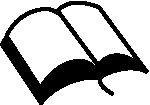
\includegraphics{booksvg.pdf}\\[4pt]
\fontfamily{lmtt}\small{Self Publishers Worldwide\\
}
\end{center}

\end{flushleft}
\end{titlepage}
\restoregeometry
% ---- End of Title Page ----

% Do not show page numbers on colophon page
\thispagestyle{empty}

\begin{flushleft}
\vspace*{\fill}
This book was typeset using \LaTeX{} software.\\
\vspace{\fill}
Copyright \textcopyright{} \the\year{}  \bookauthor\\
License: \booklicense
\end{flushleft}

% A title page resets the page # to 1, but the second title page
% was actually page 3. So add two to page counter.
\addtocounter{page}{2}


% The asterisk excludes chapter from the table of contents.
\addcontentsline{toc}{chapter}{Preface}
\chapter*{Preface}
Quantum computing and communication are hot topics. Software development kits (SDKs) including IBM Qiskit and Google Cirq have been made available to software engineers. But they are useless if the engineers are not trained with quantum algorithms and protocols, which have been described as mysterious and incomprehensible. Can engineers be taught with the algorithms and protocols without studying quantum physics? After all, the Nobel prize winning physicist and one of the best educators, Richard Feynman, says “I think I can safely say that nobody really understands quantum mechanics.”

This book says "Yes!" The only concept that one needs to learn about quantum physics is that at the minuscule scale, a wave cannot be divided into any smaller portion in terms of its energy or mass. The rest of undergraduate courses on quantum physics is about solving Schrödinger equation for electron waves and has no use to software and communication engineers. On the other hand, we use Wi-Fi, cellular, cable, and optical fiber communications daily and are already familiar with many features of radio and optical waves. Further, communication engineers are even able to invent new communication protocols using the basic concepts of communication theory without going deep into solving radio and optical wave equations. The goal of this book is to use the same basic concepts, especially the concept of modulation, to help software and communication engineers understand quantum algorithms and protocols and hopefully be able to invent new ones.

% Three-level Table of Contents
\setcounter{tocdepth}{3}
\tableofcontents

\mainmatter

\chapter{Introduction}\label{Introduction}
The advantage of quantum computing lies in the possibility of parallel computing. The use of quantum communication has been in key distribution.

\section{The power of parallel computing}
\index{Maze} problems are hard because there are too many paths to explore from the entrance to the exit. If changing the question of the problems from pinpointing the actual paths to finding the number of good paths, although seemingly dumb down, the challenge is as hard as the original. One still needs to explore all the possible paths to reach the conclusion.

\begin{figure}[ht]
%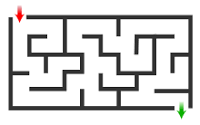
\includegraphics[width=6cm]{pic/maze.png}
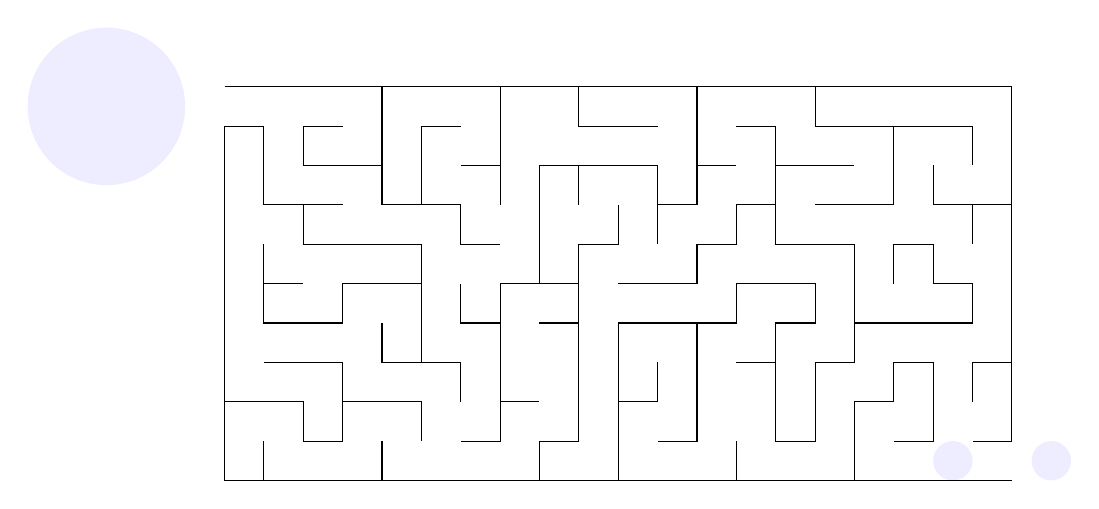
\begin{tikzpicture}[scale=0.5]
% Water
% Water
\fill[blue!7] (-3,9.5) circle (2);
\fill[blue!7] (18.5,0.5) circle (0.5);
\fill[blue!7] (21,0.5) circle (0.5);

% outer lines
\draw (0,10) -| (20,1) -- +(-1,0);
\draw (20,0) -| (0,9) -| (1,7) -- (3,7);
\draw (2,7) |- (5,6) |- (6,3) -- (6,2);
\draw (5,3) -| (4,4);
\draw (5,5) -| (3,4) -| (1,6); \draw (1,5) -- (2,5);

% bottom row
\draw (0,2) -| (2,1) -| (3,3) -- (1,3); \draw (3,2) -| (5,1);
\draw (1,0) -- (1,1);
\draw (4,0) -- (4,1);
\draw (8,0) |- (9,1) |- (10,6) -- (10,7); \draw (8,4) -- (9,4); \draw (8,5) -- (9,5);

\draw (10,0) |- (13,4) |- (15,5) |- (14,4) |- (15,1) |- (16,3) |- (14,6) |- (13,9);
\draw (10, 2) -| (11,3); \draw (12,4) |- (11,1); \draw (13,3) -- (14,3);
\draw (16,4) -| (19,5) -| (18,6) -| (17,5);
\draw (14,7) -| (13,6) -| (12,5) -- (10,5); \draw (14,8) -- (16,8);

\draw (13,0) -- (13,1);
\draw (16,0) |- (17,2) |- (18,3) |- (17,1);
\draw (20,3) -| (19,2);

% top row
\draw (4,10) |- (6,7) |- (7,6); \draw (4,8) -- (2,8) |- (3,9); \draw (5,7) |- (6,9);
\draw (7,10) -- (7,7); \draw (7,8) -- (6,8);
\draw (9,10) |- (11,9);
\draw (12,10) |- (11,7); \draw (11,6) |- (8,8) |- (7,5) |- (6,1);
\draw (12,8) -- (13,8); \draw (9,8) -- (9,7); \draw (7,4) -| (6,5); \draw (7,2) -- (8,2);
\draw (15,10) |- (19,9) -- (19,8); \draw (17,9) |- (15,7);
\draw (20,7) -| (18,8); \draw (19,7) -- (19,6);
\end{tikzpicture}
\caption{Maze}
\label{Maze}
\end{figure}

Computer scientists have long known \index{parallel computing} is the way to speed up solutions to such problems. But how to realize parallel computing needs the help of physicists. Indeed, a physicist would suggest the following experiment to attack the problem: run water into the entrance and observe what's coming out of the exit. If we see water out of the exit, we know the maze has at least one good path.

We can obtain more information if we explore the water experiment further: put several drops of water into the entrance and observe how many drops of water coming out. If three drops coming out of the exit, we can conclude that the maze has at least three good paths. We can also conclude the relative lengths of the paths by measuring the time delays of the three drops assuming water runs through all the paths at the same speed. In another word, the timing of the exiting water drops carries the length information of the paths.

One problem left is whether we can determine for sure that each of the three drops corresponds to one or more paths. For this, water is not a good medium because a water drop can always be divided up into smaller drops. Having the smallest drops, which cannot be further divided, must be included in the properties of a perfect medium for our \index{parallel computing} experiments. An ideal medium
\begin{itemize}
    \item must be able to spread and to explore all branches even to the dead-ends,
    \item must have one or more parameters, such as the time delay of a water drop, that can carry information about the lengths of the branches and the reflection of the dead-ends,
    \item can be broken up into one or more smallest drops so that information carried by the individual drops can be extracted.
\end{itemize}
Many media possess the first and even seconds. But only \index{quantum waves} possess all three.

\section{The quantum power}
 As a matter of fact, all waves are quantum waves, but we do not see the individual drops of the waves such as the radio waves transmitted by our cellphones. That is because the waves contain quadrillions of drops. We need special devices to work with the individual drops of waves. Quantum physics tells us that all waves have their smallest drops -- the \index{quanta}, which cannot be divided further in terms of their energy or mass. The very word "quantum" suggests this concept. This is the so-called particle or quantum nature of waves. Quantum physics also says that all matters including electrons and protons are fundamentally waves. Physicists refer the two concepts as the particle and wave dual-natures of matters. They are the essence of quantum physics. Their truthfulness has been proven by millions of experiments and more importantly by the successful application to the advancement of technologies especially the semiconductor and superconductor technologies.

The first hint of quantum power for parallel computing came by the proposal of the \index{Deutsch's algorithm}\cite{1985Deutsch}. The \index{Shor's algorithm}, published in 1997, is an extension of Deutsch's algorithm in scale as we will explain. But it shocks the world by its potential power of factoring large numbers and, as a consequence, breaking modern encryption technologies.

The hint of applying quantum technology to secure communication came in 1984 by the publication of the BB84 protocol\cite{BB84}. The indivisibility of a wave of one quantum prevents it from being partially tapped for eavesdropping. Further, as we will explain in the following chapter, it cannot be intercepted for eavesdropping while at the same time being reproduced for re-transmission to avoid detection because of quantum \index{no-cloning theorem}.

\subsection{The quantum nature}
To most people, particles have the image of point-like things with negligible sizes but observable locations. This image is wrong and is the cause to all the misunderstandings about quantum physics. The particle nature really refers to the fact that all matters have the smallest drops when measured by their energy or mass, and should be referred as the quantum nature. For electrons and protons, measuring their mass shows the smallest quanta. For electromagnetic waves including lights, measuring their energy shows the smallest quanta, and each quantum is called a photon.

We must remember that the only parameter that describes the quantum nature of a wave is its energy or mass. Whether it contains one quantum or more quanta of energy or mass does not change its size or location. Where it can spread to and the time delay it incurs are independent to whether it contains one quantum or more quanta of energy or mass. The quantum nature may be considered a feature of the electromagnetic waves and electron waves, which work with in quantum computing and communication. It gives us the precision needed for parallel computing. But information representation and parallel processing rely on other features of wave. Otherwise, paradoxes such as Einstein–Podolsky–Rosen (EPR) paradox \cite{EPR} are unavoidable.

\subsection{The wave nature}
When talking about waves, we often visualize ripples in a lake, or the surges in oceans and seas. We observe water being pushed up and then pulled down by gravity. If we shake one end of a string as shown in Fig. \ref{String}, we can observe closely and see that each section of the string vibrates and the \index{propagation} of the \index{vibration} from close to far. \index{Vibration} in time and \index{propagation} in space are the fundamental features of all waves. But can we consider the vibration of a guitar string a wave? Indeed, we can. The reason why we do not perceive propagation is that it gets reflected back and forth by the two fixed ends of the string. Therefore, propagation remains a defining feature of waves, even if their propagation is constrained in the spatial dimensions.

Quantum computing and communication use only electromagnetic waves and electron waves. Electromagnetic waves are the vibration of electric and magnetic fields. We are particularly familiar with radio waves and light waves used in Wi-Fi, cellular, cable, and optical fiber communications, as they are part of our daily lives. However, we do not see the quantum nature of these waves because each has quadrillions or more quanta flowing by per second. We only see the average effect.

The vibration of an electron wave is not visible as a vibrating string or directly measurable as an electromagnetic wave. But physicists do find sufficient evidence validating the Schrödinger equation that shows the vibration. And the Thomson's double slit experiment\cite{THOMSON} does show the vibration propagates. More important, the development of semiconductor and superconductor technologies is based on the understanding of the wave nature of electrons.

\begin{figure}[ht]
%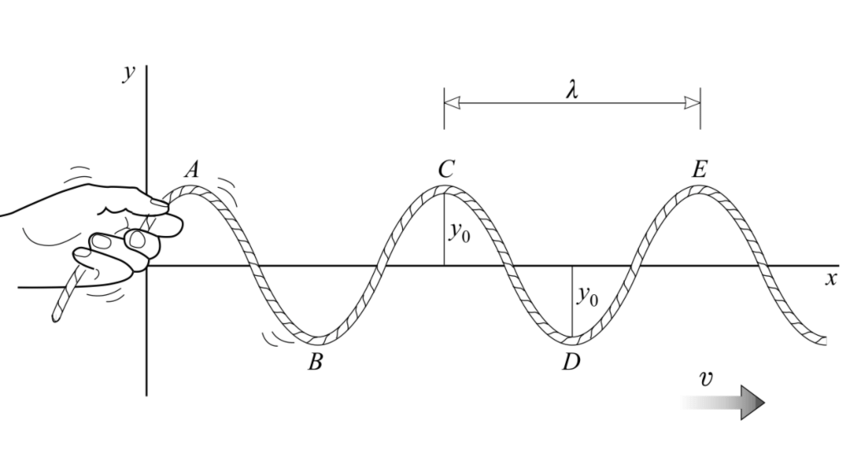
\includegraphics[width=6cm]{pic/wave-in-a-string.png}
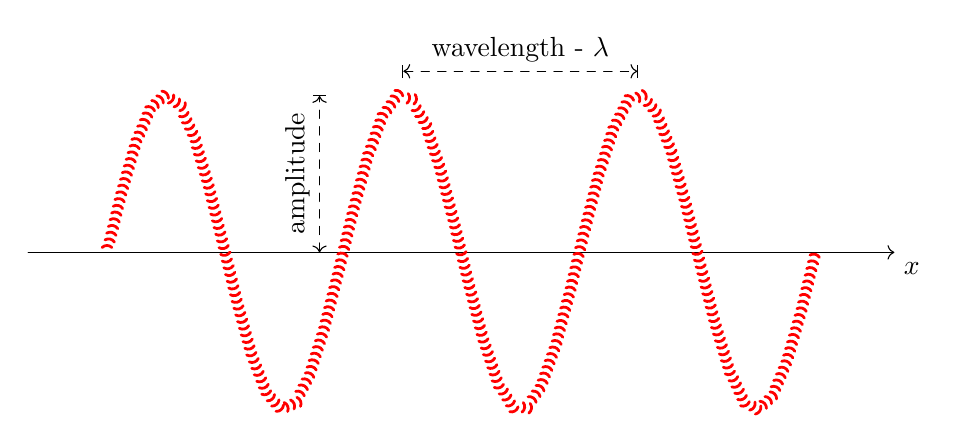
\begin{tikzpicture}[line join=round, line cap=round]

  % draw coordinate
  \draw[->] (-1,0) -- (10,0) node[pos=1.02,below] {$x$};
 % \draw[->] (0, -1) -- (0,2);
  % Rope properties
  \def\length{9}  % Length of the rope
  \def\thickness{1}  % Thickness of the rope
  \def\waveAmplitude{2}  % Amplitude of the wave
  \def\waveLength{3}  % Wavelength
  \def\segments{50}  % Number of segments
  
  % Draw the rope
  \draw[decorate, decoration={waves, segment length=2.5}, line width=\thickness, red]
    (0,0) -- plot[domain=0:\length, samples=\segments]
    (\x, {\waveAmplitude*sin(\x*(360/\waveLength))}) -- (\length,0);

    % label
    %\draw[red, fill] (3.75,2) circle(0.05cm);
    %\draw[red, fill] (6.75,2) circle(0.05cm);
    %\draw[dashed] (2,2) -- (3.75,2);
    \draw[<->|, dashed] (2.7,0) -- (2.7,2) node[pos=0.5, rotate = 90, above] {amplitude};
    \draw[|<->|, dashed] (3.75,2.3) -- (6.75,2.3) node[pos=0.5, above] {wavelength - $\lambda$};

\end{tikzpicture}
\caption{Wave arisen from shaking or vibrating a string.}
\label{String}
\end{figure}

\section{Wave and information}
\subsection{Information representation}
When we get our blood pressure measured in a doctor's office, the height of the mercury in a glass column represents the information of our blood pressure. The height of mercury in the column is what we actually measure and is what we use the height of a mercury in a cylinder to represent the information of our blood pressure. We see that physical characteristics, which can be measured in numbers, can be used to represent information.

Information theory assumes all \index{information} can be presented as numbers. The numbers, which are often called \index{symbol}s by communication engineers, in turn are mapped to physical characteristics of waves in all communication systems as well as quantum computing devices. Mapping information to numbers is called \index{encoding}, and mapping numbers to the characteristics of a wave is called \index{modulation} by communication engineers.

\begin{table}[]
\label{information-characteristics}
\begin{tabular}{|l|l|l|}
\hline
Information & Encoding numbers & Physical characteristics  \\ \hline
Blood pressure & real number & height of mercury in a cylinder \\ \hline
Picture & pixel 0 or 1 & Radio wave phase and amplitude (QAM) \\ \hline
\end{tabular}
\caption{Information represented by physical characteristics}
\end{table}

\subsection{Wave characteristics}
In Fig. \ref{String}, the height of the rope at any location $x$ along its propagation direction and time $t$ may be described as a wave function $h(x,t)$. The simplest wave function is a sinusoidal function as drawn in the figure,
\begin{equation}
    h(x,t) = A sin[2\pi (\frac x \lambda - \frac t T) +\phi]
\end{equation}
where $A$ and $\lambda$ are respectively the amplitude and the wavelength as shown in Fig. \ref{String}. $T$ and $\phi$ are the period and phase as shown in Fig. \ref{Wave}. Shown but not labeled in Fig. \ref{String} is the polarization of the vibration, which is in the $y$ direction and is perpendicular to the propagation direction. Fig. \ref{Wave} plots the height of the string vibration in the time dimension and is characterized by period and phase. All these characteristics wavelength, amplitude, period and polarization can be modulated to represent information. But period is the inverse of frequency and is also proportional to the wavelength. Changing one of the three characteristics is equivalent to changing another and is all called frequency modulation.

\begin{figure}[ht]
\begin{tikzpicture}[scale=1.2]
    \draw[->] (-3.8,0) -- (3.9, 0)  node[pos=1.02,below] {$t$};
    \draw[->] (0,-3.5) -- (0,3.5);
    \draw[dotted, red] (-3.5,0) sin (-2.5,3) cos (-1.5,0) sin (-0.5,-3) cos (0.5,0) sin (1.5,3) cos (2.5,0) sin (3.5,-3);
    \draw[red, fill] (-2.5,3) circle(0.05cm);
    \draw[red, fill] (1.5,3) circle(0.05cm);
    \draw[dashed] (-2.5,0) -- (-2.5,3) node[pos=0.5, rotate = 90, above] {amplitude};
    \draw[dashed] (-2.5,3) -- (1.5,3) node[pos=0.3, above] {period - $T$};
    \draw[red, fill] (0.5,0) circle(0.05cm);
    \draw[dashed] (0.25,-0.1) -- (1,-2) node[below] {phase};
\end{tikzpicture}
\caption{Height of the string vibration in time domain.}
\label{Wave}
\end{figure}

In radio wave communication, which includes mobile or cellphone communication we use everyday, the modulations of frequency, phase, and amplitude serves as the primary methods for information representation. In optical communication, combinations of amplitude, phase and polarization modulations are often used. In subsequent sections, we will find that quantum devices use all of these modulation schemes for information representation. A device that converts numbers to the mapped wave characteristics is called \index{modulator}, and that doing the reverse -- converting wave characteristics to numbers -- are called \index{demodulator}.

\section{Constructing a quantum system}
Like in a conventional computer, a quantum computer has memory devices too. And each memory unit is called a quantum bit or qubit, which uses  a wave of one quantum to store information. The parameters of the wave represent the the stored information. In contrast, a conventional random access memory (RAM) may use the voltage created by countless electrons accumulated at one side of the semiconductor device to represent information. A RAM can be read many times because there are countless number of electrons. A qubit, however, can only be read out once -- porting to conventional memory devices -- because there is only one quantum of wave to use.

A quantum gate, like one in a conventional computer, can read information from one or several input qubits, combine or manipulate the information, and write outcomes to output qubits. A quantum gate can read, write and manipulate information carried by a wave with one or several quanta. 

is a memory device with one quantum of a wave. Information is represented and stored by its wave characteristics. Unlike the memory devices in a conventional computer, a qubit can in theory store unlimited amount of information as we will discuss in chapter \ref{C-qi}. A quantum gate takes the wave from an input qubit, changes the wave characteristics according to the information in other qubits or conventional computer bits, and thus transform the information in the original input qubit. The transformed information may be stored in an output qubit. A measuring device, which sometimes called a measuring gate, measures the wave characteristics of an output qubit and stores in output information in conventional memory. However, the measurement involves energy exchange with the wave in the qubit and inevitably alters the wave characteristics irreversibly. Therefore, the measurement can extract at most one bit of information from the qubit, and whatever rest of information is altered to be unrecoverable. We will discuss this topic in detail in chapter \ref{C-qi}.

Quantum circuits are composed by connecting these three types of devices into functional units. Quantum computers have software that instructs gates to transform the information in the input qubits and store resulting information in the output qubits. Quantum communication systems are also constructed by the three types of devices except the qubits are communication channels instead of memory devices.

When implementing the algorithms and protocols in software, we first draw out them as quantum circuit diagrams. Our software programs would call out qubits for input and output as well as the gates for processing according to the circuit diagrams.
\begin{verbatim}
from qiskit import QuantumCircuit # and more packages if needed
N=15
a = randint(2, N) 

qc =QuantuamCircuit(N+4, N)	#N+4 qubits
For q in range(N)
  qc.h(q)		# Hadamard gate
qc.x(3+N)		# X gate
\end{verbatim}
Qubit stands for quantum bit. For quantum computing, a qubit is the data memory device that typically stores a bit of information to be processed. The storage medium is a quantum of wave, and the device includes hardware that contain the wave. For quantum communication, a qubit is the channel uses one quantum of wave to carry one bit of information. It is no difference from a radio wave or optical wave communication channel except it uses one quantum of wave at a time. Appendix \ref{A-qubit} explains the physics behind the construct and operation principles of several types of qubit devices. In Chapter \ref{C-qi} on quantum information, we will revise the notion that a qubit can stores or carries only one-bit of information. Before that, we will stay with the qubit definition implied by its name and repeated in literature.

Conventional computers have no resemblance to quantum computers. Even before the appearance of modern computer, the not widely known subject of optical computing has explored the parallel computing capability of optical waves with Fourier transformation. But its application is limited and has not become a subject of learning by many. On the other hand, quantum devices have much in common with radio and optical communication devices because they all work with waves. Radio-wave communication including mobile communication and Wi-Fi is the dominating way for everyone connecting to the wired world. Mobile devices already take advantage of waves' parallel exploration capability for transmitters and receivers to find each other. The backbone of the wired world, on the other hand, is all optical fibers. The knowledge of wave communication reaches more engineering students than quantum physics and is most relevant not only to quantum communication but also to quantum computing. This chapter reviews some of the relevant subjects of communication theories especially on modulation before delving into the following chapters on the specifics of quantum communication and computing.

At the top level, a communication system has an information sender, a channel and a receiver. The sender contains modulators that transfer information in the form of numbers to characteristics of waves and send the waves to the channel. The receiver has demodulators that translate wave characteristics back to information. In a quantum system, the modulators and demodulators are quantum gates. The information bits carried in a quantum channel are called qubits -- short for quantum bits.

An ideal channel maintains the form and shape of the waves so that no information is lost. The equivalent in a computing system is a memory device, which receives bits of information from a writer and conveys them to the reader. Channels and memory devices, which work with quantum waves, are all qubit devices and may often be loosely referred as qubits.

Quantum gates are modulators and demodulators, and are not the same as transistor gates in a conventional computer. They convert information from one form of wave to another. A circuit of quantum gates would turn a maze of data (information) to an obvious form for easy extraction and achieve the task of computation. Or a circuit can turn the data (information) to an obscure form and achieve the task of secure communication.

When we talk about quantum computers, we should understand that we don't have entire computers made of all quantum devices. They will only have some chips or co-processors be replaced by chips of integrated circuits of quantum devices. Even our conventional computers have graphic processor units (GPU) in addition to the central processing units (CPU) to help speed up the processing of video display data.

\chapter{Using waves to represent information}

In the study of communication, modulation is the subject devoted to how information being represented by physical characteristics of waves. The wealth of knowledge can be applied to not only quantum communication protocols but also to quantum computing.

Radio broadcasts first used radio waves' amplitudes to represent the volume of one's voice. This is the so called amplitude modulation (AM). The amplitude is the maximum of the vibrating electric field of the vibration instead of the maximum height of a string vibration shown in Fig. \ref{String}. Frequency modulation (FM) was later found less prone to noise in the airways than AM. That is why we now have both AM and FM on the panels of our radios. Modern radio communications, Wi-Fi and cellular, mostly use quadrature amplitude modulation (QAM) -- a combination of amplitude modulation and phase modulation (PM). Modern optical fiber communication also brings polarization modulation into the mix.

Quantum devices, working with the smallest quanta of waves, use many of modulation schemes invented for communication with their own twist. Understanding how modulation works in quantum devices is the critical link for engineers to understand quantum technologies.

\section{Phase modulation}
In chapter \ref{Introduction}, the time delays of water drops traveling through the maze channels can be used to represent information. The phase of a wave reflects the relative time delay of its propagation. Phase modulation is to use a wave's phase to represent information. The phase, usually noted with symbol $\varphi$, can take up the value of any real number in the range [0, 2$\pi$). Phase modulation is essential in every type of qubits, but it always works in combination with another type of modulation as we will see in the following sections.

\subsection{Graphical depiction of phase modulation}
In communication textbooks, we pair the amplitudes and phases of waves as polar coordinates to plot the modulation points and call the plot a constellation diagram. Such diagrams give us the most intuitive understanding of modulations involving amplitudes and phases. With phase modulation, the amplitude is a constant, let's say $A$. Naturally, the modulation points all fall on the circle of radius $A$ as shown in red in Fig. \ref{PM}.

%\node [constellation_cir] at (0,0) {};
\begin{figure}[ht]
\begin{tikzpicture}
    \draw[->] (-3.5,0) -- (3.5, 0);
    \draw[->] (0,-3.5) -- (0,3.5);
    \draw[dotted, red] (0,0) circle(3cm);
    \draw[red, fill] (30:3) circle(0.05cm);
    \draw[dashed] (1,0) arc (0:30:1) node[right, pos=0.6]{$\varphi$ - phase};
    \draw[dashed] (30:0.1) -- (30:2.9) node[pos=0.5, rotate = 30, above] {amplitude};
\end{tikzpicture}
\caption{Constellation diagram of phase modulation}
\label{PM}
\end{figure}

\subsection{Mathematical notation of phase modulation}
We can use the polar coordinate $(A, \varphi)$ as we do when plotting the constellation diagram in Fig. {PM} to represent a modulation point. We can also use complex number $A e^\varphi$ to represent a modulation point. Further, we can choose any two orthogonal vectors in the diagram as the horizontal and vertical axles, and the modulation point can be written in Cartesian coordinate as $(A cos\varphi, A sin\varphi)$.

\subsection{Digital modulation}
In the real world, communication channels and information processing devices have noises and errors. For the fidelity of information transmission, we can only select the modulations points spaced apart by the maximum of the noises and errors. Therefore, we can only use a finite number of modulations points, which may be mapped to integer numbers to represent information. This is what we call digital modulation. Modulations that can represent real numbers are called analog modulations.

All computers use digital technology if we ignore the history of using the slide rule calculators. Even abacuses are digital calculators. Communication systems however are slow to convert to digital technology. that is because for a long time, communication was mostly about voice communication -- radio broadcast and telephones, and noises and errors could be tolerated. For digital information, modulations such as AM, FM and PM often carry different names, e.g. amplitude-shift keying (ASK), frequency-shift keying (FSK) and phase-shift keying respectively (PSK).

\subsection{Channel capacity and Hartley's law}
For a communication channel, channel capacity is the maximum possible bits per second of a communication channel. When modulation is limited by noises and errors, only maximum of $M$ possible symbols -- mapped to modulation points -- can be transmitted per time slot. Assume, the communication protocol divides each second into $R$ time slots, Hartley's law gives the channel capacity to be
\begin{equation}
    C = R ln M.
\end{equation}
In theory, the maximum value of $R$ is the frequency of the carrier wave. Shannon's law relating channel capacity to signal to noise retio can easily be derived from Hartley's law if we assume noise is the only limiting factor.

In a computer memory device, the number of modulation points $M$ is the amount of information that it can store. Convert to number of bits, it can store $ln M$ bits of information.

\section{Quadrature phase-shift keying}
Quadrature phase-shift keying (QPSK) is a digital phase modulation that demonstrates many principles used in quantum devices. It uses modulation points with phases 90 degree apart. A simple choice is to use $\phi = 0, 90, 180$, and $270$ degrees to represent 2-bit symbols -- 0, 1, 10, and 11 in binary. Fig-\ref{QPSK} is its constellation diagram.

\begin{figure}[ht]
\begin{tikzpicture}
    \draw[->] (-3.5,0) -- (3.5, 0);
    \draw[->] (0,-3.5) -- (0,3.5);
    \draw[dotted, red] (0,0) circle(3cm);
    \draw[red, fill] (3,0) circle(0.05cm) node[below right] {0};
    \draw[red, fill] (0,3) circle(0.05cm) node[above right] {1};
    \draw[red, fill] (-3,0) circle(0.05cm) node[above left] {10};
    \draw[red, fill] (0,-3) circle(0.05cm) node[below left] {11};
\end{tikzpicture}
%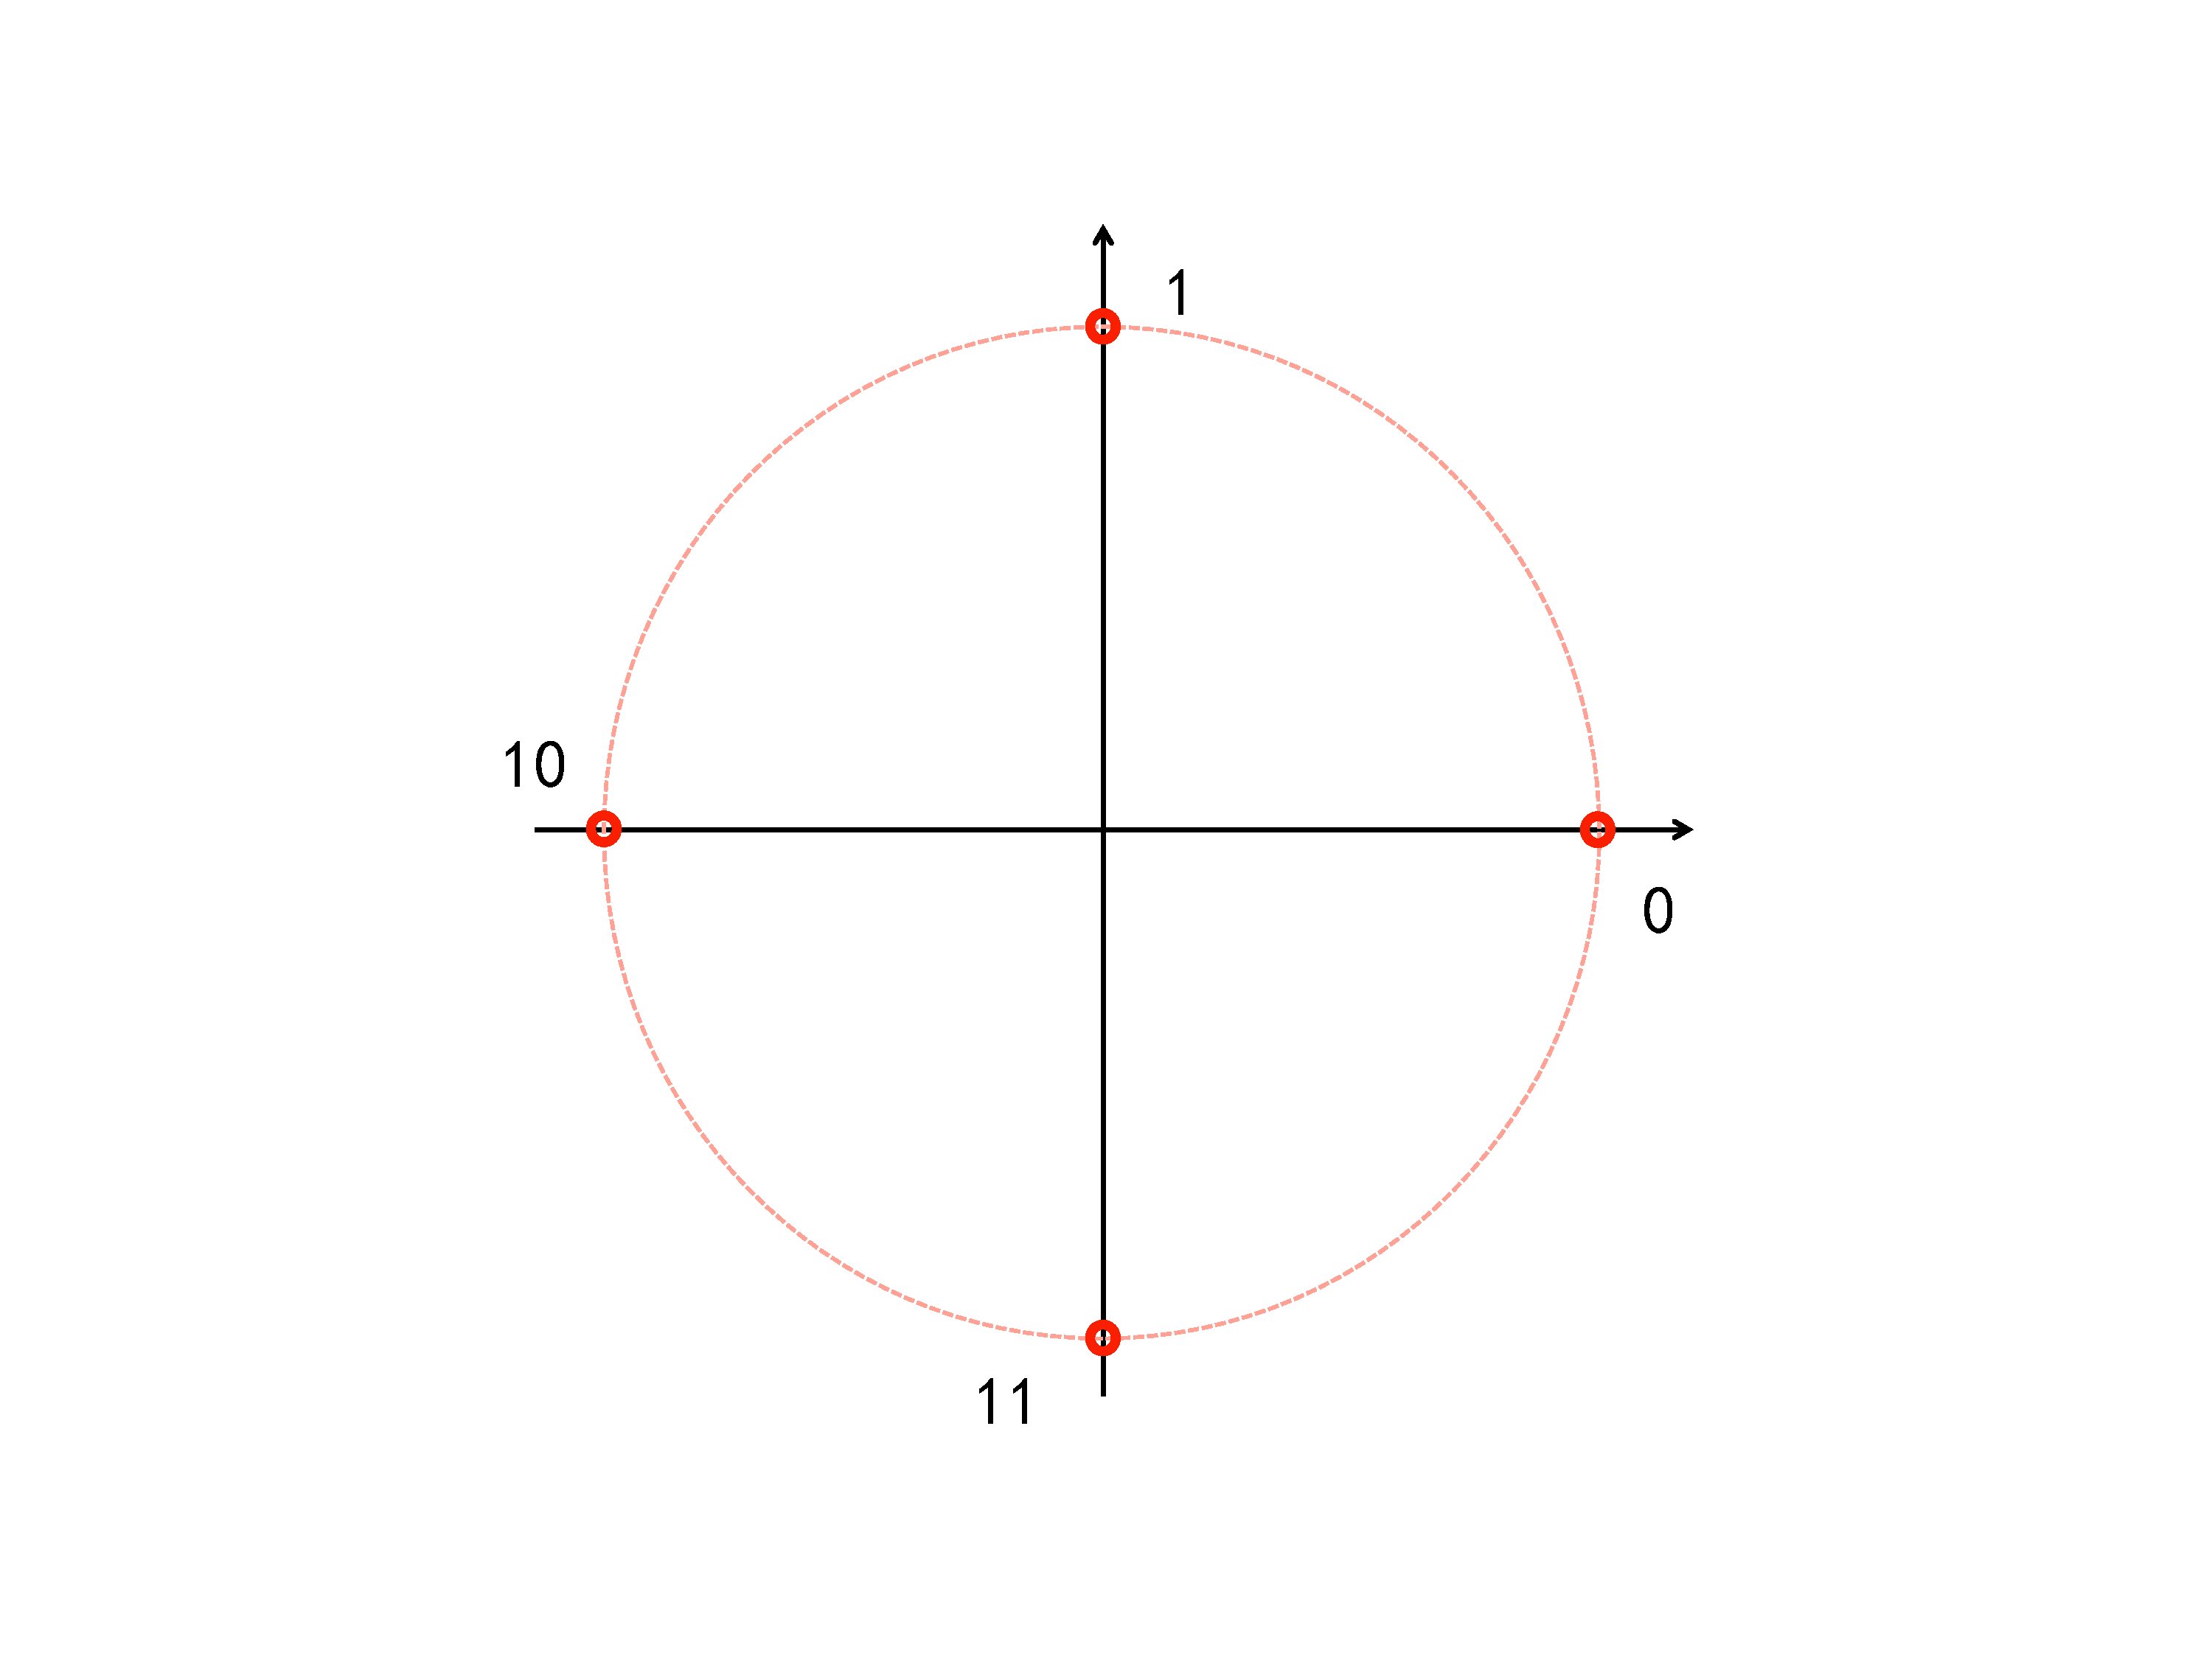
\includegraphics[width=6cm]{pic/4qpsk.pdf}
\caption{QPSK constellation diagram}
\label{QPSK}
\end{figure}

Communication engineers call the wave with zero degree phase the quadrature wave and the one with $90^\circ$ phase the in-phase wave. And they find any two waves with $90\circ$ phase difference have zero overlap during measurement assuming that the waves have the same polarization. Zero overlap results in the least probability of mistaking one wave with another during measurement. If the electric fields of two waves of the same polarization are written in their wave functions as $E_1 (x,t)$ and $E_2 (x,t)$, their overlap is defined as
\begin{equation}
    \int_{0}^{T_m} E_1 (x,t) E_2 (x,t) dt,
\end{equation}
and we will see the reason when we describe the demodulation of QPSK in section \ref{Demodulation}.

If we write out the quadrature and in-phase waves in their wave functions,
\begin{equation}
    E_q (x,t) = A sin[2\pi(\frac x \lambda - \frac t T)] and
    E_i (x,t) = A sin[2\pi(\frac x \lambda - \frac t T)+90] = A cos[2\pi(\frac x \lambda - \frac t T)],
\end{equation}
their zero overlapping is obvious.

Communication engineers also find that a wave of any phase $\varphi$ is a mixture of the quadrature and in-phase waves,
\begin{equation}
    E (x,t) = A sin[2\pi(x-f t)+\varphi] = A cos\varphi sin [2\pi (x-ft)] + A sin\varphi cos [2\pi (x-ft)].
\end{equation}
If we consider a wave represented in the constellation diagram as a vector, the quadrature wave is a vector in the horizontal axis, and the in-phase wave is in the vertical axis. The wave at any of the modulation points in Fig. \ref{PM} with phase $\varphi$ can be represented in this Cartesian coordinate as $(A cos\varphi, A sin\varphi)$. Further, this  coordinate is easiest to be expressed as a complex numbers,
\begin{equation}
    A cos\varphi + i A sin\varphi  = A e^{i\varphi}.
\end{equation}

\subsection{Symmetric QPSK}
For simpler modulator and demodulator circuitry, the symmetric QPSK modulation scheme shown in the constellation diagram Fig. \ref{sQPSK} is more widely used in practice. The modulation points are $\varphi = 45, 135, 225$ and $315$ degrees.
\begin{figure}[hb]
\begin{tikzpicture}
    \draw[->] (-3.5,0) -- (3.5, 0);
    \draw[->] (0,-3.5) -- (0,3.5);
    \draw[dashed] (2.5,2.5) -- (0, 0);
    \draw[dotted, red] (0,0) circle(3cm);
    \draw[red, fill] (2.12,2.12) circle(0.05cm) node[right] {11};
    \draw[red, fill] (-2.12,2.12) circle(0.05cm) node[above] {01};
    \draw[red, fill] (2.12,-2.12) circle(0.05cm) node[below] {10};
    \draw[red, fill] (-2.12,-2.12) circle(0.05cm) node[left] {00};
    \draw[dashed] (1,0) arc (0:45:1) node[right, pos=0.6]{$\varphi=45\circ$};
\end{tikzpicture}
\caption{Practical QPSK constellation diagram}
\label{sQPSK}
\end{figure}

\subsection{QPSK modulator and wave mixing}\label{modulation}
A practical QPSK modulator circuit is shown in Fig. \ref{Modulator}. It uses one wave generator and splits the carrier wave into two waves of equal amplitudes. One of the half becomes the in-phase wave after a 90-degree phase shifter while the other half remains as the quadrature wave. Let's assume the wave out of the generator has a wave function
\begin{equation}
    A sin 2\pi(\frac x \lambda - \frac t T),
\end{equation}
and the quadrature and in-phase waves are
\begin{equation}
    \frac A {\sqrt 2} sin 2\pi(\frac x \lambda - \frac t T) and \\
    \frac A {\sqrt 2} cos 2\pi(\frac x \lambda - \frac t T).
\end{equation}
On the path of each of the wave, a 180-degree phase shifter is placed. But in each time slot, a two-bit number, say $b_1 b_0$ in binary, is fed into the modulator with each bit turning on-and-off one of the phase shifters. When the two waves are summed up by the mixer, the output wave should be
\begin{equation}
    \frac A {\sqrt 2} sin[2\pi(\frac x \lambda - \frac t T)+b_0 \pi] +
    \frac A {\sqrt 2} cos[2\pi(\frac x \lambda - \frac t T)+b_1 \pi] \\
    =\frac A {\sqrt 2} (-1)^{b_0} [sin 2\pi(\frac x \lambda - \frac t T) +
     (-1)^{(b_1-b_0} cos 2\pi(\frac x \lambda - \frac t T)] \\
    =\frac A sin [2\pi(\frac x \lambda - \frac t T) +\frac \pi 4 +b_0 \frac \pi 2+b_1 \frac \pi]
    \frac A {\sqrt 2} (-1)^{b_1} cos 2\pi(\frac x \lambda - \frac t T).
\end{equation}
Actually, it'd be much easier if we use the complex number notation to calculate the resulting wave:
\begin{equation}
    \frac A {\sqrt 2} e^{i b_0 \pi} + \frac A {\sqrt 2} e^{i b_1 \pi + i \frac \pi 2} \\
    = \frac A {\sqrt 2} (-1)^{b_0}[1+i (-1)^{(b_1-b_0)}]\\
    = A  e^{i(b_0 \pi + (b_1 - b_0) \frac \pi 4)}.
\end{equation}

modified scheme: in every time slot, 2 bits are fed into the modulator. Each bit is used to modulate a base carrier wave's phase. The two base carrier waves are orthogonal, one of zero phase and the other of 90-degree in phase. If the input to a carrier is "0", its phase is shifted another 180 degrees. The combined or summed up wave of the two carriers is the output of the modulator going into the communication channel. The constellation diagram this scheme is shown in Fig. \ref{QPSK}.

We see that one wave from the source can be divided up into two waves, which can then be combined into one after modulation. In fact, all waves can be combined into one and may be regarded as one wave if they are coherent with each other -- their phases are correlated. Combination, mixing or composing several waves into one is the same concept as superposition in quantum physics although the latter refers to combination, mixing or composition of waves with equal number of quanta.

\begin{figure}[ht]
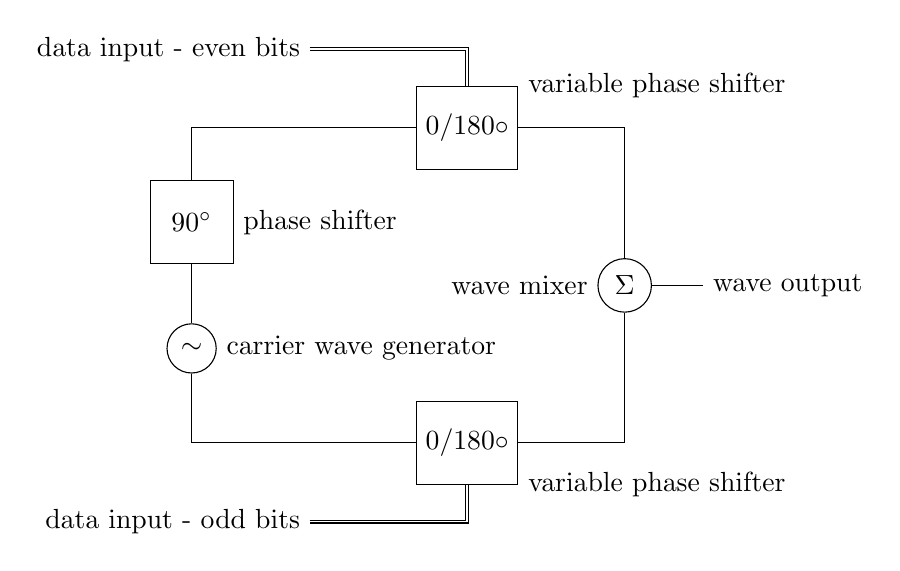
\begin{tikzpicture}
    \path %(-5,0) node[anchor=east] (start) {Wave} 
    (-3.5,-0.8) node[circle, draw=black] (lo) {$\sim$}
    (-3.5,0.8) node[Gate] (p90) {$90^\circ$}
    (0,2) node[Gate, text width=30] (tm) {$0/180\circ$}
    (0,-2) node[Gate, text width=30] (bm) {$0/180\circ$}
    (2,0) node[circle, draw=black] (add) {$\Sigma$}
     (3,0) node[anchor=west] (output) {wave output};
    \draw (lo.east) node[anchor=west] {carrier wave generator};
    \draw (add.west) node[anchor=east] {wave mixer};
    \draw (p90.east) node[anchor=west] {phase shifter};
    \draw (tm.north east) node[anchor=west] {variable phase shifter};
    \draw (bm.south east) node[anchor=west] {variable phase shifter};
    \draw (lo) -- (p90) |- (tm) -| (add);
    \draw (lo) |- (bm) -| (add);
    \draw (add) -- (output);
    \path (-2,3) node[anchor=east] (even) {data input - even bits}
    (-2,-3) node [anchor=east] (odd) {data input - odd bits};
    \draw[double] (even) -| (tm);
    \draw[double] (odd) -| (bm);
\end{tikzpicture}
\caption{QPSK modulator circuit}
\label{Modulator}
\end{figure}

\subsection{Demodulation and wave splitting}\label{Demodulation}
Fig. \ref{deodulator} shows a demomulator circuit, which reverses the modulation:
- the received signal wave is divided into two waves;
- each is mixed with one of the two orthogonal waves, which are from the same local source
- The the proportions of the two resonations determine the phase angle of the incoming wave. Bit numbers are output according to the phase angle.

\begin{figure}[ht]
%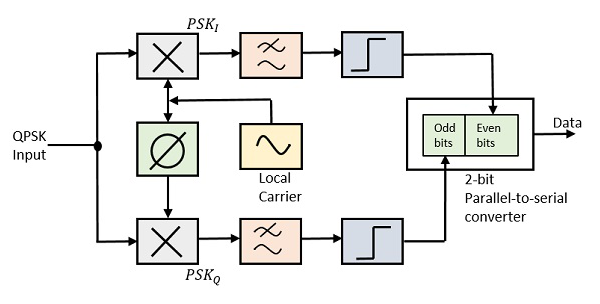
\includegraphics[width=6cm]{pic/qpsk_demodulator.jpg}
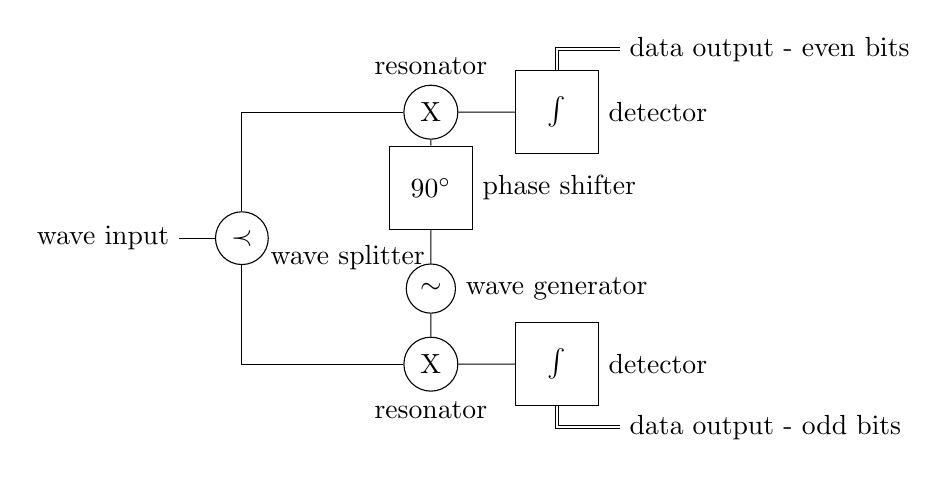
\begin{tikzpicture}[scale=0.8]
    \path
    (0,-0.8) node[circle, draw=black] (lo) {$\sim$}
    (0,0.8) node[Gate] (p90) {$90^\circ$}
    (0,2) node[circle, draw=black] (ta) {X}
    (0,-2) node[circle, draw=black] (ba) {X}
    (2,2) node[Gate] (tm) {$\int$}
    (2,-2) node[Gate] (bm) {$\int$}
    (-3,0) node[circle, draw=black] (split) {$\prec$}
     (-4,0) node[anchor=east] (input) {wave input};
    \path (3,3) node[anchor=west] (even) {data output - even bits}
    (3,-3) node [anchor=west] (odd) {data output - odd bits};

    \draw (lo.east) node[anchor=west] {wave generator};
    \draw (p90.east) node[anchor=west] {phase shifter};
    \draw (tm.east) node[anchor=west] {detector};
    \draw (bm.east) node[anchor=west] {detector};
    \draw (ta.north) node[anchor=south] {resonator};
    \draw (ba.south) node[anchor=north] {resonator};
    \draw (bm) -- (ba) -- (lo) -- (p90) -- (ta) -- (tm);
    \draw[double] (even) -| (tm);
    \draw[double] (odd) -| (bm);

    \draw (ba) -| (split)  |- (ta);
    \draw (split.south east) node[anchor=west] {wave splitter};
    \draw (split) -- (input);    
\end{tikzpicture}
\caption{QPSK demodulator circuit}
\label{deodulator}
\end{figure}

\section{Polarization modulation}
For an electromagnetic wave, the vibration of its electric field is always perpendicular to its direction of propagation just like the vibration of a string. Polarization modulation is used in modern optical fiber communication in combination with QPSK. The combined modulation is called dual polarization quadrature phase shift keying (DP-QPSK). As with phase modulation, any two waves whose polarizations are orthogonal to each other have the least overlap and can be distinguished the best during measurement.

\begin{figure}[ht]
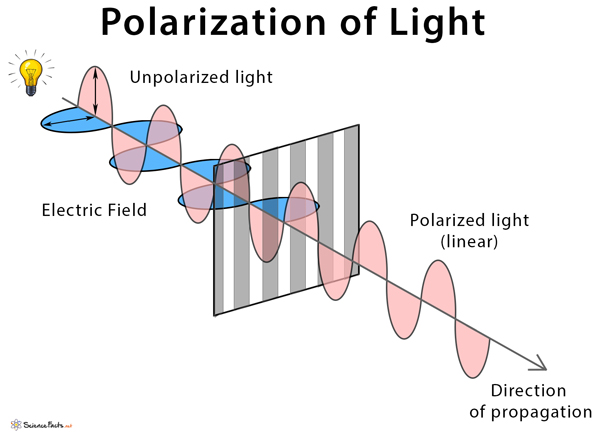
\includegraphics[width=10cm]{pic/Polarization-of-Light.jpg}
\caption{Polarization}
\label{Polarization}
\end{figure}

\begin{figure}[ht]
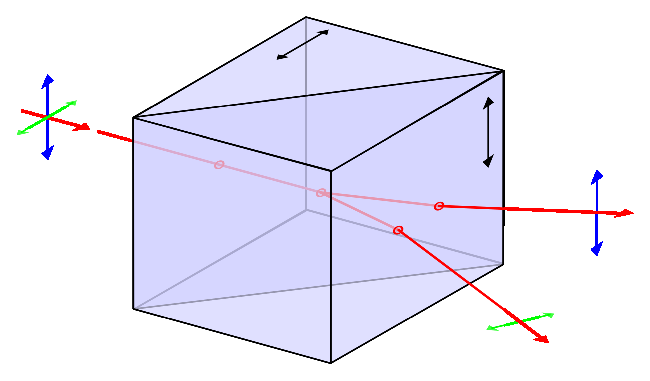
\includegraphics[width=12cm]{pic/Wollaston-prism.eps}
\caption{Polarization beam splitter}
\label{Polarizer}
\end{figure}

Free space communication is mostly used for satellites to communicate with each other. There is no substance in space to degrade the power of the light wave. The receiver may as receive less power if the light beam diverge in a large angle. Laser lights are typically used. Free space communication can also be used for ship-ship communication if the distance is not too far resulting in high power loss.

Lights are propagating electromagnetic waves and obviously are best suited for communications. The vibration direction of the electric field of an electromagnet wave is its polarization. A free space optical qubit uses one optical wave of horizontal polarization to represent the binary number 0 and is thus label $\keta{0}$. It uses the one of vertical polarization to represent 1 and is labeled $\keta{1}$. The two waves have the same frequency and amplitude. They are orthogonal to each other of course. A wave of polarization angle $\theta_p$ can be considered the superposition of the two base waves: the $\keta{0}$ wave contributes $cos\theta_p$ amount in amplitude while the $\keta{1}$ wave contributes $sin\theta$.

Polarization modulation is also used in optical fiber communication. For example, dual polarization quadrature phase shift keying (DP-QPSK) modulation is a widely used.

\section{Optical waveguide qubits and gates}
Another type of qubits uses lights confined in optical waveguides or fibers. We use the optical wave in waveguide A to represent the binary number 0 and label it $\keta{0}$. We use the one in waveguide B to represent 1 and label it $\keta{1}$. The two waves have the same frequency and amplitude. They don't overlap and are of course orthogonal to each other. If we bring the two waveguides together to overlap (using an optical coupler), we get a superposition wave that is a sum of both waves. If the sum has $cos\theta$ amount in amplitude from $\keta{0}$ wave contributes and $sin\theta_p$ amount in amplitude from the $\keta{1}$ wave, we can use the value $\theta_p$ to characterize the superposition wave.

\begin{figure}[ht]\label{Fiber}
%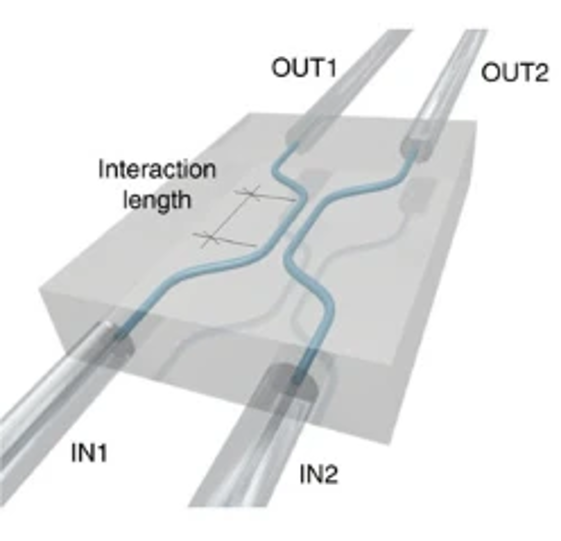
\includegraphics[width=6cm]{pic/wguideQubit.png}
%\caption{Waveguide qubit}
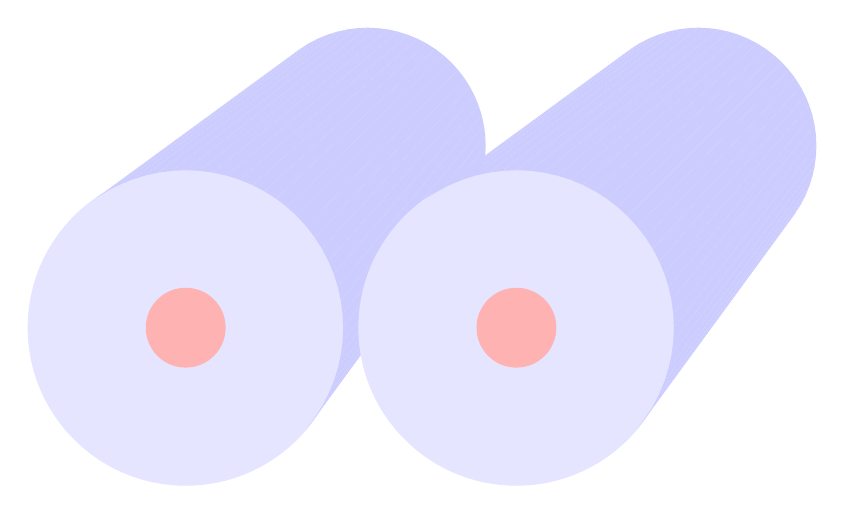
\begin{tikzpicture}[scale=0.5]
    \def\R{4} % Outer radius
    \def\Rb{3} % Outer radius
    \def\r{1} % Inner radius
    \def\L{6} % Half Length of the tube
    \def\S{4.2} % half Shift distance between tubes
    \def\I{5} % increment

    % Left tube
    \draw[blue!10,fill] (-\S,0,\L) circle (\R);   
    \draw[red!30,fill] (-\S,0,\L) circle (\r);    
    %\draw[decorate,decoration=zigzag] (-\S,0,-\L) circle (\Rb);
    \foreach \t in {-40,-35,...,123} {
        \fill[blue!20] ({\R*cos(\t+\I)-\S}, {\R*sin(\t+\I)}, \L) -- ({\R*cos(\t)-\S}, {\R*sin(\t)}, \L) 
        -- ({\Rb*cos(\t)-\S}, {\Rb*sin(\t)}, -\L) -- ({\Rb*cos(\t+\I)-\S}, {\Rb*sin(\t+\I)}, -\L) -- cycle;
    }

    % Right tube    
    \draw[blue!10,fill] (\S,0,\L) circle (\R);   
    \draw[red!30,fill] (\S,0,\L) circle (\r);    
    %\draw[black!10] (\S,0,-\L) circle (\Rb);
    \foreach \t in {-40,-35,...,123} {
        \fill[blue!20] ({\R*cos(\t+\I)+\S}, {\R*sin(\t+\I)}, \L) -- ({\R*cos(\t)+\S}, {\R*sin(\t)}, \L) 
        -- ({\Rb*cos(\t)+\S}, {\Rb*sin(\t)}, -\L) -- ({\Rb*cos(\t+\I)+\S}, {\Rb*sin(\t+\I)}, -\L) -- cycle;
    }
\end{tikzpicture}
\caption{A waveguide qubit comprised by two single-mode optical fibers}
\end{figure}

\section{Optical waveguide quantum computing chip}
If we take a look at the Xanadu.ai M-8 quantum computing chip, we see it very much ressembles a maze. The optical waveguides are the paths that light waves traverse. Its couplers and splitters ressemble the junctions of maze. A coupler merge two light paths into one, and a splitter split one into two. The chip has 8 entrances and 8 exits and can build $8^8$ possible paths.

Quantum physics tells us that all matters are waves and in addition, they all have the smallest quanta, which cannot be divided finer when measured in their energy or mass. A wave, like water, can spread in space and propagate in time through all possible paths and give us the power of parallel computing. The drop-like behavior gives us the needed precision. Physicists refer the drop-like behavior the particle nature of matters. But the term particle unavoidably suggests minuscule in size and clarity in trajectory, and leads to avoidable puzzles and paradoxes with waves' spread in space and propagation in time. We should imagine or interpret electrons and electromagnetic waves like water drops: they can spread in space and propagate in time, may be subjected to constraints such as reflective objects, but show the smallest quanta when measured by energy or mass.

\section{Superconductor qubits}
A superconductor transmon qubit is similar to the string of a guitar and uses the first two standing waves, which resonate at the first and second harmonic frequencies respectively, to represent the integers of "0" and "1". Such a qubit is constructed by two superconductors separated by a layer of insulator. The insulator is thin enough for electrons to move ("tunnel") back and forth from one superconductor to another without loss of energy. But traveling through the insulator leads to delays (phase delays) of the electrons. The back-and-forth movement (vibration) of the electrons between the two superconductors resonate as standing waves at periods fractions of the delay. typically, the first fundamental frequency and the first harmonic are used to represent "0" and "1".
\begin{figure}[ht]
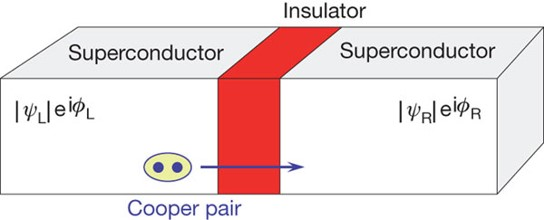
\includegraphics[width=12cm]{pic/supercQubit.jpg}
\caption{Josephson junction}
\label{Superconductor}
\end{figure}

\begin{figure}[ht]
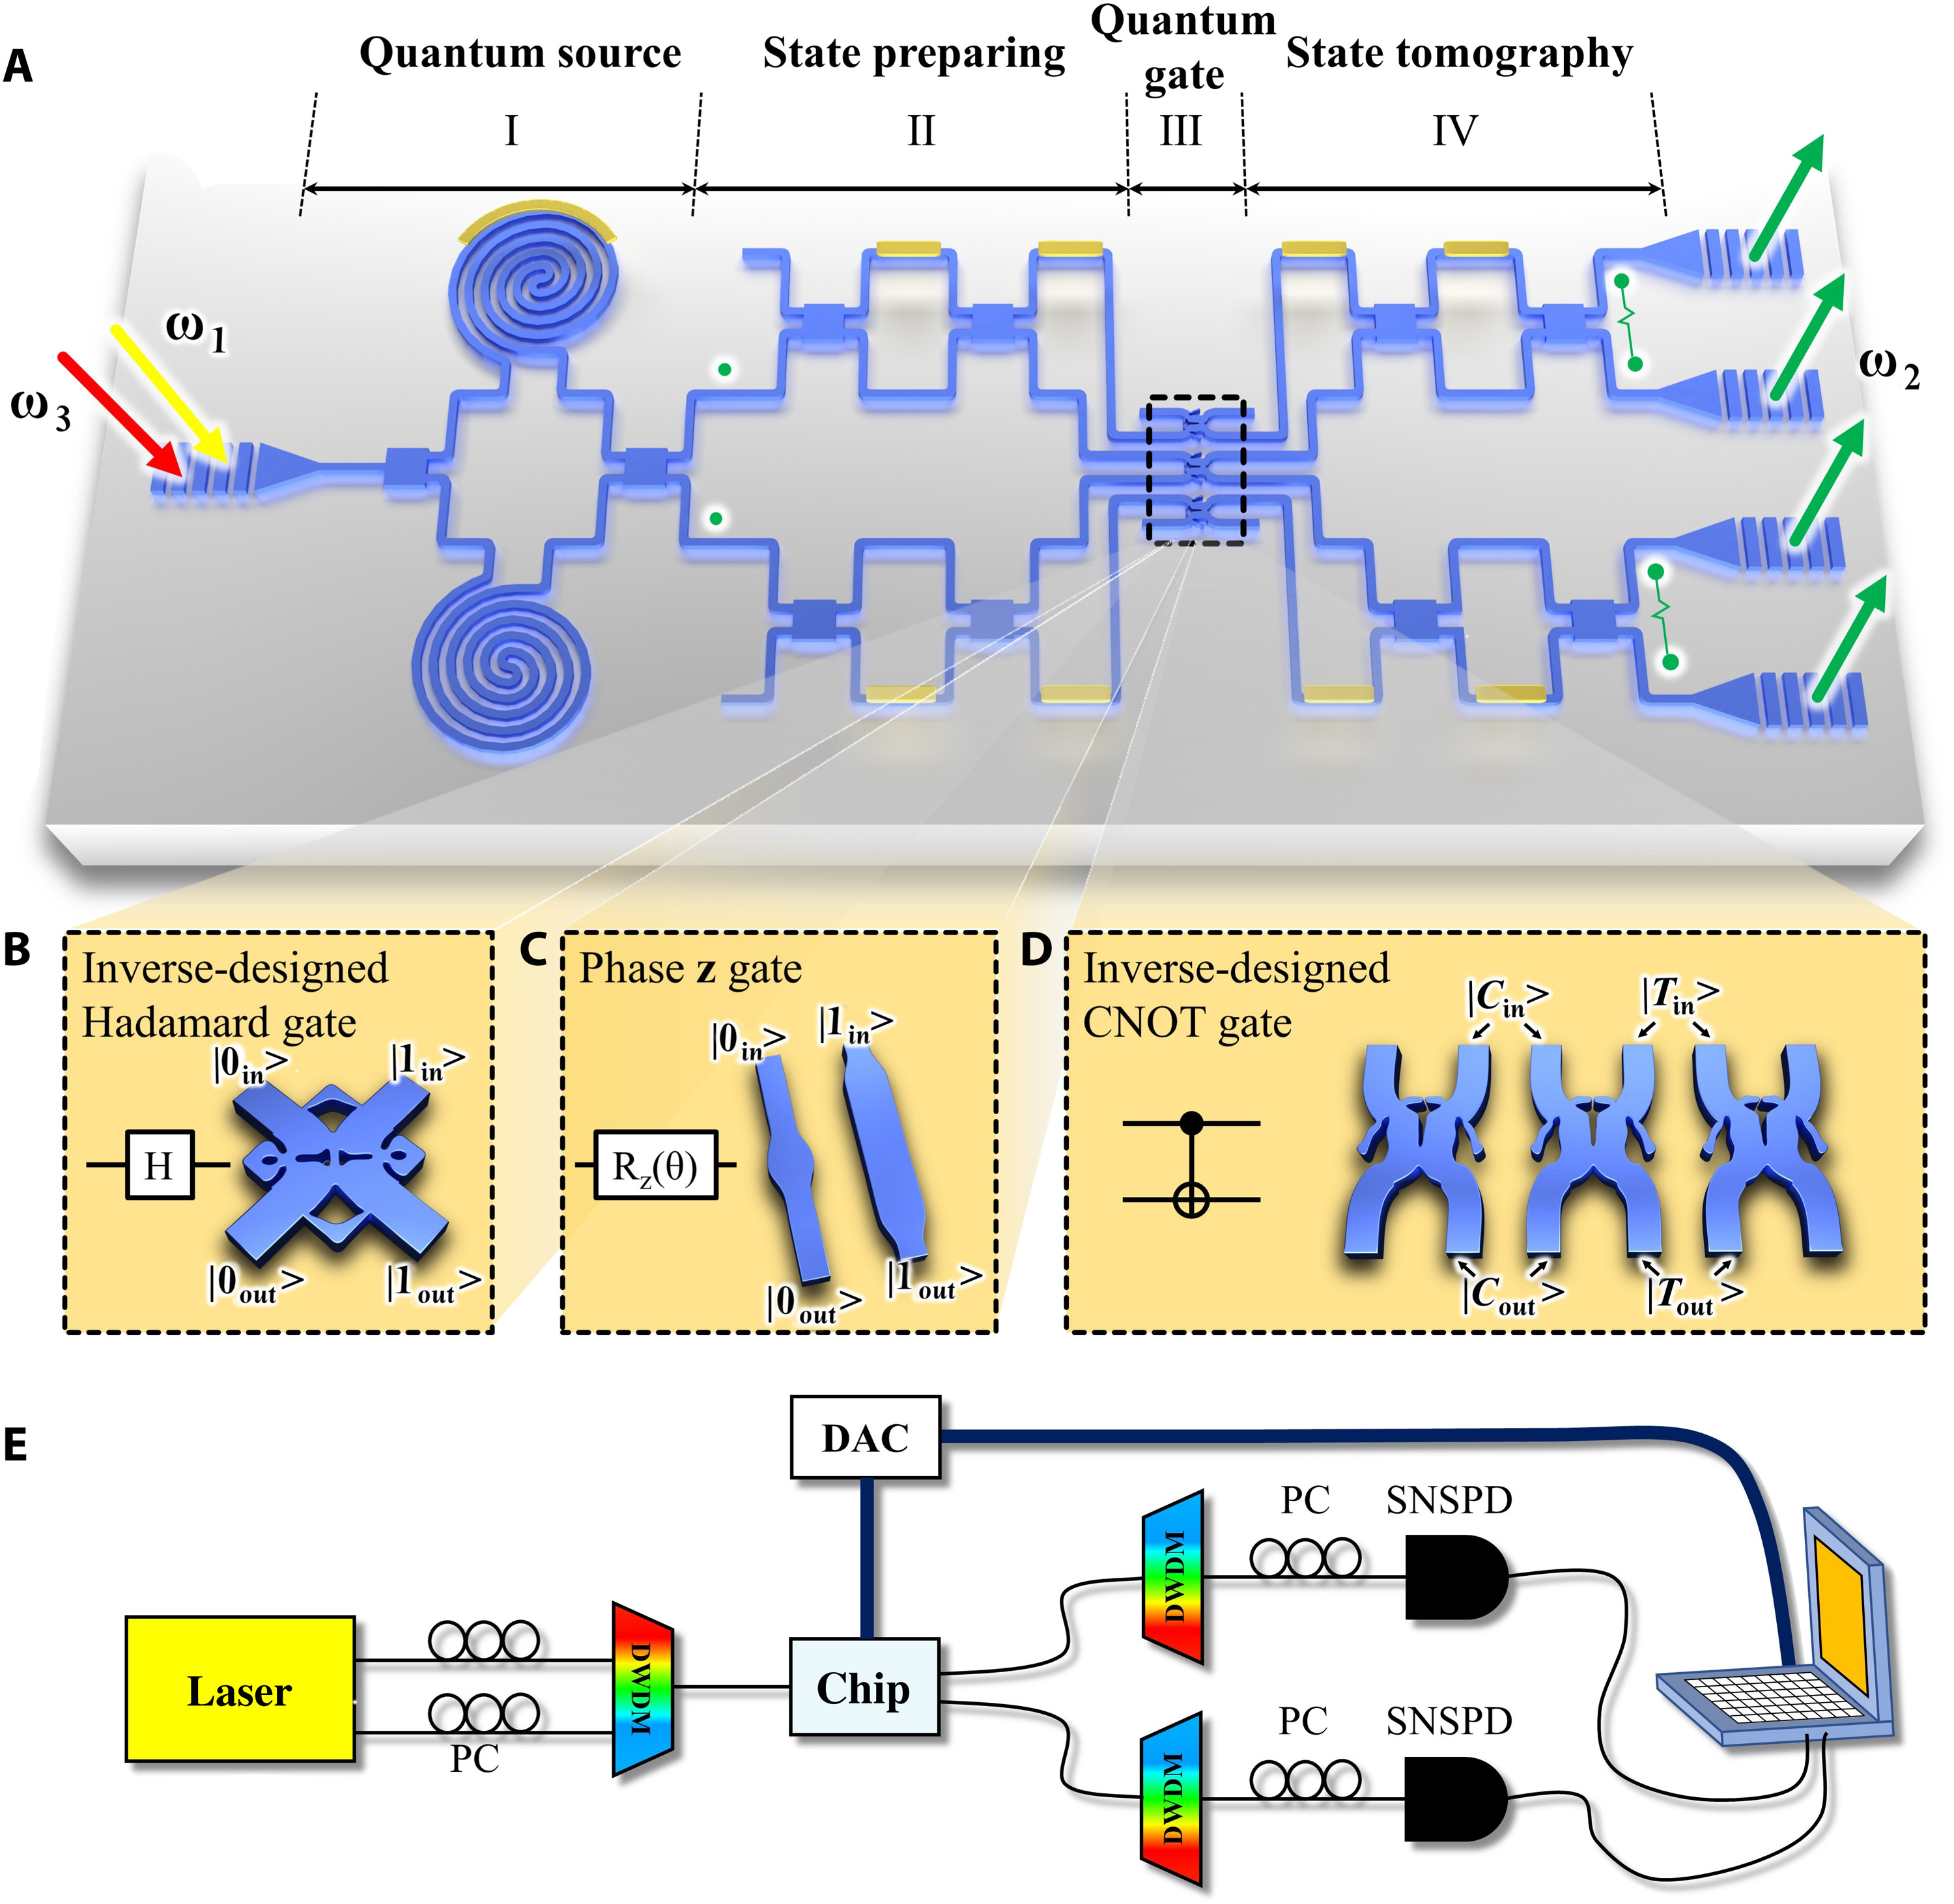
\includegraphics[width=12cm]{pic/superGates.jpg}
\caption{Superconductor gates.}
\label{superGates}
\end{figure}

\section{Quadrature amplitude modulation}
Quadrature amplitude modulation (QAM) is a combination of amplitude modulation and phase modulation. Modern radio communication such as Wi-Fi and mobile communications all use the digital forms of QAMs.
\begin{figure}[ht]\label{QAM}
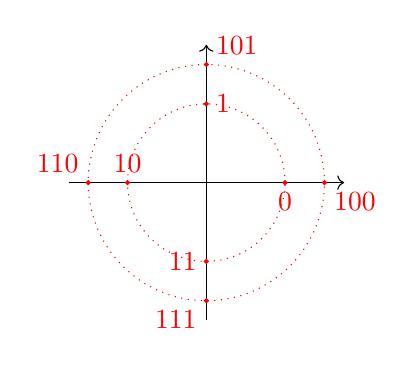
\begin{tikzpicture}[scale=0.5]
    \draw[->] (-3.5,0) -- (3.5, 0);
    \draw[->] (0,-3.5) -- (0,3.5);
    \draw[dotted, red] (0,0) circle(2cm);
    \draw[dotted, red] (0,0) circle(3cm);
    \draw[red, fill] (2,0) circle(0.05cm) node[below] {0};
    \draw[red, fill] (0,2) circle(0.05cm) node[right] {1};
    \draw[red, fill] (-2,0) circle(0.05cm) node[above] {10};
    \draw[red, fill] (0,-2) circle(0.05cm) node[left] {11};
    \draw[red, fill] (3,0) circle(0.05cm) node[below right] {100};
    \draw[red, fill] (0,3) circle(0.05cm) node[above right] {101};
    \draw[red, fill] (-3,0) circle(0.05cm) node[above left] {110};
    \draw[red, fill] (0,-3) circle(0.05cm) node[below left] {111};
\end{tikzpicture}
\begin{tikzpicture}\label{8QAM}
    \draw[->] (-3.5,0) -- (3.5, 0);
    \draw[->] (0,-3.5) -- (0,3.5);
    \draw[dashed] (2.5,2.5) -- (-2.5,-2.5);
    \draw[dashed] (-2.5,2.5) -- (2.5,-2.5);
    \draw[dotted, red] (0,0) circle(2cm);
    \draw[dotted, red] (0,0) circle(3cm);
    \draw[red, fill] (45:2) circle(0.05cm) node[above left] {11};
    \draw[red, fill] (135:2) circle(0.05cm) node[above right] {01};
    \draw[red, fill] (225:2) circle(0.05cm) node[above left] {00};
    \draw[red, fill] (-45:2) circle(0.05cm) node[above right] {10};
    \draw[red, fill] (45:3) circle(0.05cm) node[right] {111};
    \draw[red, fill] (135:3) circle(0.05cm) node[left] {101};
    \draw[red, fill] (225:3) circle(0.05cm) node[left] {100};
    \draw[red, fill] (-45:3) circle(0.05cm) node[right] {110};
\end{tikzpicture}
\caption{Constellation diagrams of two 8QAM systems}
\end{figure}

\section{Frequency modulation}
Frequency reflects how fast the vibration of a wave is. In radio communication, frequency is used for \index{multiplexing} -- having several waves of different frequencies to share the same propagating medium i.e. the airway so that multiple channels can be transmitted over the same medium at the same time. On the receiving end, different channels are separated out according to the frequencies of the waves. This type of technology is called \index{multiplexing}. Each wave, which carries one stream of information, is called a \index{channel}.

\chapter{Quantum information}\label{C-qi}
\section{Quantum concepts}
For engineers, only two concepts of quantum physics are needed: 1. all matters are waves even the seemingly size-less electrons and protons are; 2. all waves have their smallest drops, which cannot be divided. Physicists refer the two concepts the partical and wave duality of matters. The first concept tells us that, not limited to radio and optical waves, electrons and protons can also be used to make qubits. However, the implication of the second concept is far more profound and is not explored by traditional communication theory. One implication is that analog amplitude modulation is not possible because amplitude depends on the number of quanta in the wave and can only be use for digital modulation. Second, each qubit can only be measured once.

\section{Quantum measurement}
The quantum nature is not shown until a wave is measured. The concept is simple, but leads to profound differences between measure a quantum wave and a classical wave. The most profound difference is that one quantum of a wave can only be measured once. After measurement, the quantum of wave is no longer the same as it once was. This is the so-called Bohr quantum collapse theory. Another difference is the possible values of measurement are limited to the eigen-values, which may be a concept foreign to engineering students. The differences are natural results of von Neumann's projection theory of measurement -- a highly abstract mathematical theory. To engineers, however, quantum measurement may be better understood as demodulation and resonance as described in the next chapter. 

\subsection{Limitation of measurement}
The final stage of demodulation involves measuring the wave's mass or energy. The result is always a discrete number -- 1, 2, ..., or $n$ -- quanta of mass or energy. The amplitude of the wave is usually proportional to the square root of the mass or energy and takes only discrete values although not exactly 1, 2, ... or $n$.

Measurement always involve energy or mass exchange between the wave and the measurement apparatus. When measuring a photon, for example, its energy is transferred to an electron, and the movement or change in the electron induces an electrical current observable to humans. Lost all the energy to the electron, the photon is "annihilated" -- in physicists' lingo -- and cannot be measured again. The unique feature of quantum information is that we can modulate a qubit device as much information as the cardinal of real numbers but that we can only measure at most once per quantum.

\subsection{Quantum terminology}
By tradition, physicists keep on using the term particle, which may cause the biggest confusion. To most people, particles have the image of point like or of negligible sizes. Physicists believed electrons were point-like in size when JJ Thomson discovered them in 1897. But when Ernest Rutherford discovered atomic nucleus 14 years later, people raised the question: why is the size of an atom much bigger than that of its nucleus? Why wouldn't the tiny negatively charged electrons fall into the positively charged nucleus and be combined into an atom close to the size of the nucleus -- if it were to happen, we would have not seen the world as we have.

Physicists refer the drop-like behavior of electrons and all other matters as the particle behavior. "Quantum" should have been the perfect word in place of particle, but we think "drop" is a better word for non-physicists to understand.

Beside particle, physicists use the term "state" to refer the wave of one drop. It is the same concept as "mode" in the context of optical communication and photonics. It is used to describe a wave when the absolute amplitude value is known or unimportant. But the term carries many different meanings to engineers. We will believe it's wise to use the term "wave" in place of state. By tradition, physicists use the so-called Dirac "bra-ket" notation to label quantum states. In the ket notation, the base carrier waves are noted as $\keta{0}$ and $\keta{1}$.

When talking about electrons being waves, people are often puzzled and ask what is vibrating in an electron wave. Physicists are puzzled too and have been debating the possibilities without conclusion. Engineers don't have to interject into the debate and need only know that an electron wave qubit has frequency, phase and polarization for modulating.

\section{Qubit modulation}
\subsection{Requirements on modulation}
We have two conflicting requirements when considering how to modulate a qubit:
\begin{itemize}
    \item For parallel computing/exploration, the modulation points should be as many as possible.
    \item For output, the measurable modulation points are limited to the "0" and "1" points.
\end{itemize}

The first requirement is easy to understand, and phase modulation, with modulation points $\phi \in [0, 2\pi)$, meets the requirement. The second requirement is due to that fact that one qubit has only one quantum of wave, which resonates with only one of the local oscillators in the demodulator as shown in Fig. \ref{deodulator} and never both.

As described in the Appendix on qubit devices, all devices add a second modulation such as polarization, frequency, mode modulation or the like to meet the second requirement. In this book, we refer these secondary modulations a generic term, $\theta$ modulation, because all of them can be characterized by an angle value $\theta \in (-\pi/2, \pi/2]$ as discussed in the appendix on qubit devices.

\subsection{Measurable modulation points}
\subsubsection{Quadrature amplitude modulation}
Since a wave is in quanta, 1, 2, 3, ..., or n quanta, its amplitude is discrete too although not in increment of 1, 2, 3, ..., or n. Adding amplitude modulation is by adding more qubits and can be used only for digital modulation. Amplitude modulation is always used to add code points for digital modulation and cannot be used for parallel computing.

\subsection{Analog modulation}
Analog modulation can only be used at input or in processing. For communication, each qubit actually has two channels -- $\theta$ and $\varphi$. And their channel capacities per qubit duty cycle are $\theta \in (-\pi/2, \pi/2] and \varphi \in [0, \pi)$. For computing, that is the capacities are the amount of information a qubit can store.

\subsection{Demodulation and quantum measurement}
When a cellphone receives a radio wave, the demodulator can divide the wave into many portions to measure the amplitudes and phases. But with a qubit, although we can adopt any of the modulation technique and put information in any of the data points $(\theta, \varphi)$, we cannot divide one quantum of wave for multiple measurement.

Similar to a demodulator of QPSK. a demodulator of a qubit expose the quantum of wave to two electronic resonators orthogonal to each other.  If we know the qubit is modulated by BQSK, detecting the qubit in the $\keta{0}$ wave means the qubit's phase $\theta = 0$. Further, the absence of detecting signal in the $\keta{1}$ wave also suggests $\theta = 0$ too. But if the qubit is originally modulated in any other way, we have no way of measuring the knowing the information that the qubit represents. the probability of one resonator responds to the wave depends on how much the resontor overlaps with the wave in space and time.

In contrast to conventional communication and computing systems, information entered into a quibit may be lost at demodulation or measurement. That is the unique feature of quantum information.

\subsection{Wave characteristics for qubit modulation}
\begin{table}[]
\caption{Wave characteristics for qubit modulation}
\label{modulation-characteristics}
\begin{tabular}{lll}
Wave parameters &Represented numbers &Qubit design   \\
Amplitude & Number of qubits 1, 2, ... & all qubits \\
Phase & $\varphi \in (-\pi /2, \pi /2] $& all qubits \\
Frequency & $\theta \in (-\pi /2, \pi /2]$ & SC-IBM, Google; trapped ion - IonQ \\
Mode & $\theta \in (-\pi /2, \pi /2]$ & Xanadu, PsiQuantum \\
Polarization & $\theta \in (-\pi /2, \pi /2]$ & USTC \\
Spin & $\theta \in (-\pi /2, \pi /2]$ & 
\end{tabular}
\end{table}

\section{Mathematical notation of qubit modulation}
From communication theory perspective, a qubit is best described by the parameter pair $(\theta, \varphi)$. But other notations developed by physicists may be easier to use when working on problems involving more than one qubit. 
\subsection{Ket notation}
Summing up the base carriers, the superposition wave can be noted as $\keta{s} = cos{\theta} \keta{0} + e^{i \varphi} sin{\theta} \keta{1}$ or simply $\keta{s} = a \keta{0} + b \keta{1}$. Here, the $+$ sign means wave addition but has no mathematical meaning. And $a$ and $b$ are complex numbers and reflect the amplitude and phase contributions to the superposition. Even with the constraint $|a|^2+ |b|^2$, this notation includes waves $e^{i\lambda} (cos{\theta} \keta{0} + e^{i \varphi} sin{\theta})$ which are the same except their global phase $\lambda$.

\subsection{Vector notation}
For mathematicians and computer scientists, the physical meaning of wave addition can be ignored, and the vector notation $
\begin{pmatrix}
    a \\
    b
\end{pmatrix}$ is best for derivation and calculation.

But not all of the 4 real numbers the two complex numbers can be used independently for modulation. First, the amplitude of the wave is one to be sure that the qubit contains only one quantum $|a|^2 + |b|^2 = 1$.
\begin{equation}
    \begin{pmatrix}
    cos\theta & -e^{i\lambda} sin\theta \\
    e^{i\varphi} sin\theta & e^{i(\varphi + \lambda)} cos\theta
\end{pmatrix}
\end{equation}
Any operation rotates the data point of a qubit on the Bloch sphere and can be described by the triplet of Euler angles, $\delta \theta, \delta \varphi, \delta \lambda$. The matrix notation is
\begin{equation}
    \begin{pmatrix}
        cos\delta \theta & -e^{i\delta \lambda} sin\delta \theta \\
        e^{i \delta \varphi} sin\delta \theta & e^{i \delta \varphi+ \delta \lambda} cos\theta 
    \end{pmatrix}
\end{equation}

\subsection{Binary numbers}

If we measure waves in any other way than space or time, we find their smallest "drops" -- the particle nature of matter. Quantum physics started a hundred years ago when Einstein first proposed that electromagnetic waves, when measured in their energy, have the smallest drops called photons.

When measuring in electric charge, physicists discovered the smallest drops first and call them electrons before they realized their wave nature.

Measurement is the very thing that the quantum world is different from the classical world. In the quantum world, with an article, you only have one chance to measure it.)

Digital technologies gain precision over analog technologies but lose in the amount of information they can carry. The amount of information that a modulation technique can carry relates to the size or cardinality of the set of numbers that it can represent. With analog PM, the cardinality of the set [0, 2$\pi$) is infinity and is the same as the entire set of real numbers. But the set of integers that a digital modulation represent is finite. And the amount of information that a digital communication channel carries per time slot is finite. To increase the communication speed, the cellphone industry has been trying to squeeze more and more information per time slot by adopting increased data points of QAM modulations -- 4QAM, 8QAM, 16QAM ....
From the above description of the various types of qubits, we see that they all have the pseudo phase $\theta_p$ to characterize the 
orthogonality or overlap among the waves in the polarization, spatial or frequency domains, and can be used represent real numbers in the $\{\theta_p \in [0, \pi/2)\}$ domain. In addition, the relative phase in the time domain of the two base carrier waves in a qubit is another independent variable that can be. Physicists usually use $\theta_q = \theta_p/2 \keta{0}$ and the Bloch sphere as in Fig. \ref{bloch} to draw an intuitive picture of the entire modulation domain of a qubit $\{\theta_q \in [0, \pi]$ and $\phi \in [0, 2\pi)\}$.

\begin{table}[]
\caption{Parameters and ranges for modulation}
\label{modulation-parameters}
\begin{tabular}{|l|l|l|}
\hline Parameter &Represented numbers &Note                 \\
\hline Amplitude &Number of qubits $\in \{1, 2, 3, ...\}$   & None \\
\hline Phase & $\varphi \in (-\pi /2, \pi /2] $& Z gate \\
\hline Polarization angle (spatial overlap) & $\theta \in (-\pi /2, \pi /2]$ &X gate \\
\hline
\end{tabular}
\end{table}

\section{Graphical depictions}
\subsection{Quarter sphere diagram}
%\begin{figure}[ht]
%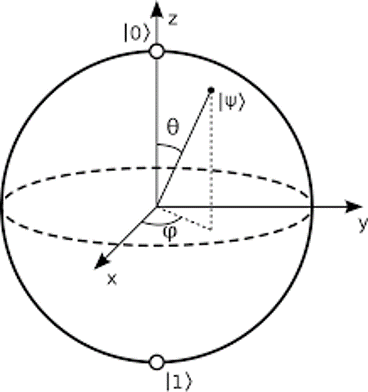
\includegraphics[width=6cm]{pic/blochSphere.png}
%\caption{Bloch sphere}
%\label{Bloch}
%\end{figure}

\begin{figure}[ht]
\tdplotsetmaincoords{0}{0}
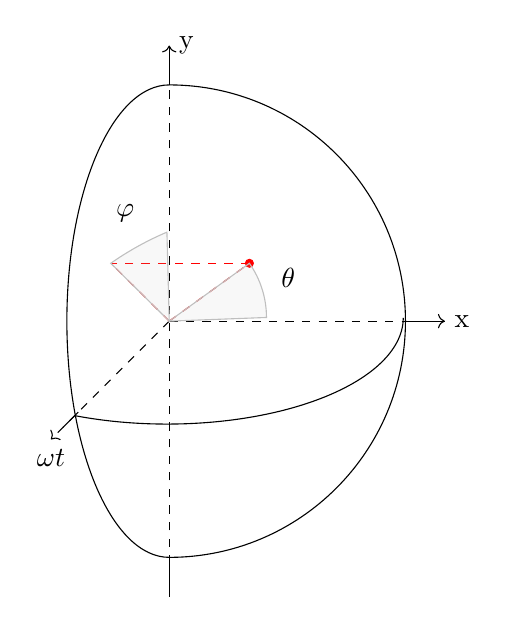
\begin{tikzpicture} %[scale=2,tdplot_main_coords]
 \def\rvec{3}
 \def\thetavec{50}
 \def\phivec{40}
 
    %Axes
    \coordinate (O) at (0,0,0);
    \draw[dashed, ->] (0,0,0) -- ++(3.5, 0,0) node[below,right] (x) {x};
    \draw[dashed, ->] (0,-3.5,0) -- ++(0, 7, 0) node[above,right] (y) {y};
    \draw[dashed, ->] (0,0,0) -- ++(0, 0, 3.9) node[below] (z) {$\omega t$};
    \draw[] (0,-3) arc(-90:90:3 and 3);
    \draw[] (0,3) arc (90:270:1.3 and 3);
    \draw[] (-1.2,-1.2) arc (-113:0:3 and 1.35);
    \draw[] (3,0,0) -- ++(0.5, 0, 0);
    \draw[] (0,-3.5,0) -- ++(0, 0.5, 0);
    \draw[] (0,3,0) -- ++(0, 0.5, 0);
    \draw[] (0,0,3) -- ++(0, 0, 0.5);

    % Vector
    \tdplotsetcoord{P}{\rvec}{\thetavec}{\phivec}
    \draw[red,fill] (P) circle(0.05);
    \draw[dashed, red] (O) -- (P) node[circle] (Ptheta) {};
    \draw[dashed, red] (O) -- (Pyz) node[circle] (Pphi) {};
    \draw[dashed, red] (P) -- (Pyz);
    %\draw[dashed, red] (Px) -- (Pxz);

    % angles;
    \draw [shift={(0,0)}, lightgray, fill, fill opacity=0.1] (0,0) -- (P) arc (35:0:1.2) -- cycle;
    \draw [shift={(0,0)}, lightgray, fill, fill opacity=0.1] (0,0) -- (Pyz) arc [start angle=125, delta angle=-12, radius=3.9 ] -- cycle;
    %\draw [shift={(0,0)}, lightgray, fill, fill opacity=0.1] (0,0) -- (Pyz) arc (75:60:1.2) -- cycle;
    \draw( -0.8, 1.6) node[anchor=north west] {$\varphi$};
    \draw( 1.3, 0.8) node[anchor=north west] {$\theta$};
\end{tikzpicture}
\caption{Qubit modulation space}
\label{bloch-alt}
\end{figure}

\subsection{Bloch sphere}
\begin{figure}[ht]
\tdplotsetmaincoords{0}{0}
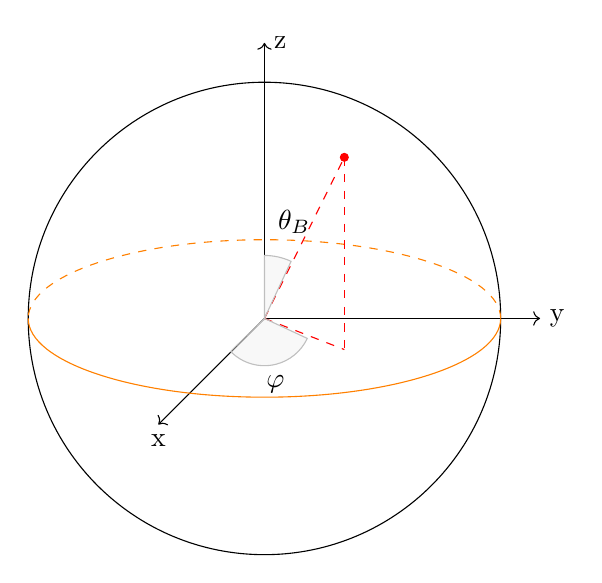
\begin{tikzpicture} %[scale=2,tdplot_main_coords]
 \def\rvec{3}
 \def\thetavec{70}
 \def\phivec{60}
 
    %Axes
    \coordinate (O) at (0,0,0);
    \draw[->] (0,0,0) -- ++(3.5, 0,0) node[below,right] (y) {y};
    \draw[->] (0,0,0) -- ++(0, 3.5, 0) node[above,right] (z) {z};
    \draw[->] (0,0,0) -- ++(0, 0, 3.5) node[below] (x) {x};
    \draw[] (0,0) circle(3);
    \draw[orange] (-3,0) arc (180:360:3 and 1);
    \draw[dashed, orange] (3,0) arc (0:180:3 and 1);

    % Vector
    \tdplotsetcoord{P}{\rvec}{\thetavec}{\phivec}
    \draw[red,fill] (P) circle(0.05);
    \draw[dashed, red] (O) -- (P) node[circle] (Ptheta) {};
    \draw[dashed, red] (O) -- (Pxz) node[circle] (Pphi) {};
    \draw[dashed, red] (P) -- (Pxz);
    %\draw[dashed, red] (Px) -- (Pxz);

    % angles;
    \draw [shift={(0,0)}, lightgray, fill, fill opacity=0.1] (0,0) -- (65:0.8) arc (65:90:0.8) -- cycle;
    \draw [shift={(0,0)}, lightgray, fill, fill opacity=0.1] (0,0) -- (-135.7:0.6) arc (-135.7:-25:0.6) -- cycle;
    \draw( -0.1, -0.6) node[anchor=north west] {$\varphi$};
    \draw( 0.05, 1.5) node[anchor=north west] {$\theta_B$};
\end{tikzpicture}
\caption{Bloch sphere}
\label{bloch}
\end{figure}

\subsection{Constellation diagrams}
Constellation diagrams are familiar to engineers and are great graphical illustration of modulations involving only phase and amplitude. But quantum devices add $\theta$ modulation.

\section{Mostly used modulation points}\label{Sec-Plus}
\subsection{$\keta{1}$}
$\keta{1}$ is one of the base waves of a qubit. However, quantum computing circuit diagrams usually assume all input waves are $\keta{0}$, and assume a $\keta{1}$ wave being transformed by an X gate from a $\keta{0}$ wave --
$\keta{1} = X \keta{0}$ -- in ket notation. In vector notation, the $X$ gate has a matrix representation
\begin{equation}
    X = \begin{pmatrix}
        0 & 1 \\
        1 & 0
    \end{pmatrix}.
\end{equation}
In circuit notation,
\begin{figure}[ht] \label{X1}
\begin{quantikz}
    \lstick{\ket{0}} & \gate{X} & \qw \rstick{\ket{1}}
\end{quantikz}
\caption{Use X gate to produce $\keta{1}$ wave.}
\end{figure}
The X gate can also be represented as $\bigoplus$. But in this book, we do not use this notation.

We see that an X gate flips the bases $\keta{0}$ and $\keta{1}$ from one to another. 

\subsection{The $\keta{+}$ and $\keta{-}$ waves}
To read out from a qubit, it must be in a binary modulation. Similar to QPSK shown in Fig. \ref{qQPSK}, we can map the modulation points $\theta=0$ and $\pi/2$ to represent "0" and "1" respectively as shown in the constellation diagram Fig. \ref{QPSK} 
\begin{figure}[hp]
\begin{tikzpicture}
    \draw[->] (-3.5,0) -- (3.5, 0);
    \draw[->] (0,-3.5) -- (0,3.5);
    \draw[dashed] (2.5,2.5) -- (0,0);
    \draw[dashed] (0,0) -- (2.5,-2.5);
    \draw[dotted, red] (0,0) circle(3cm);
    \draw[red, fill] (3,0) circle(0.05cm) node[below right] {0};
    \draw[red, fill] (0,3) circle(0.05cm) node[above right] {1};
    \draw[red, fill] (2.12,2.12) circle(0.05cm) node[right] {+};
    \draw[red, fill] (2.12,-2.12) circle(0.05cm) node[below] {-};
    \draw[dashed] (1,0) arc (0:45:1) node[right, pos=0.6]{$\theta=\pi/4$};
\end{tikzpicture}
%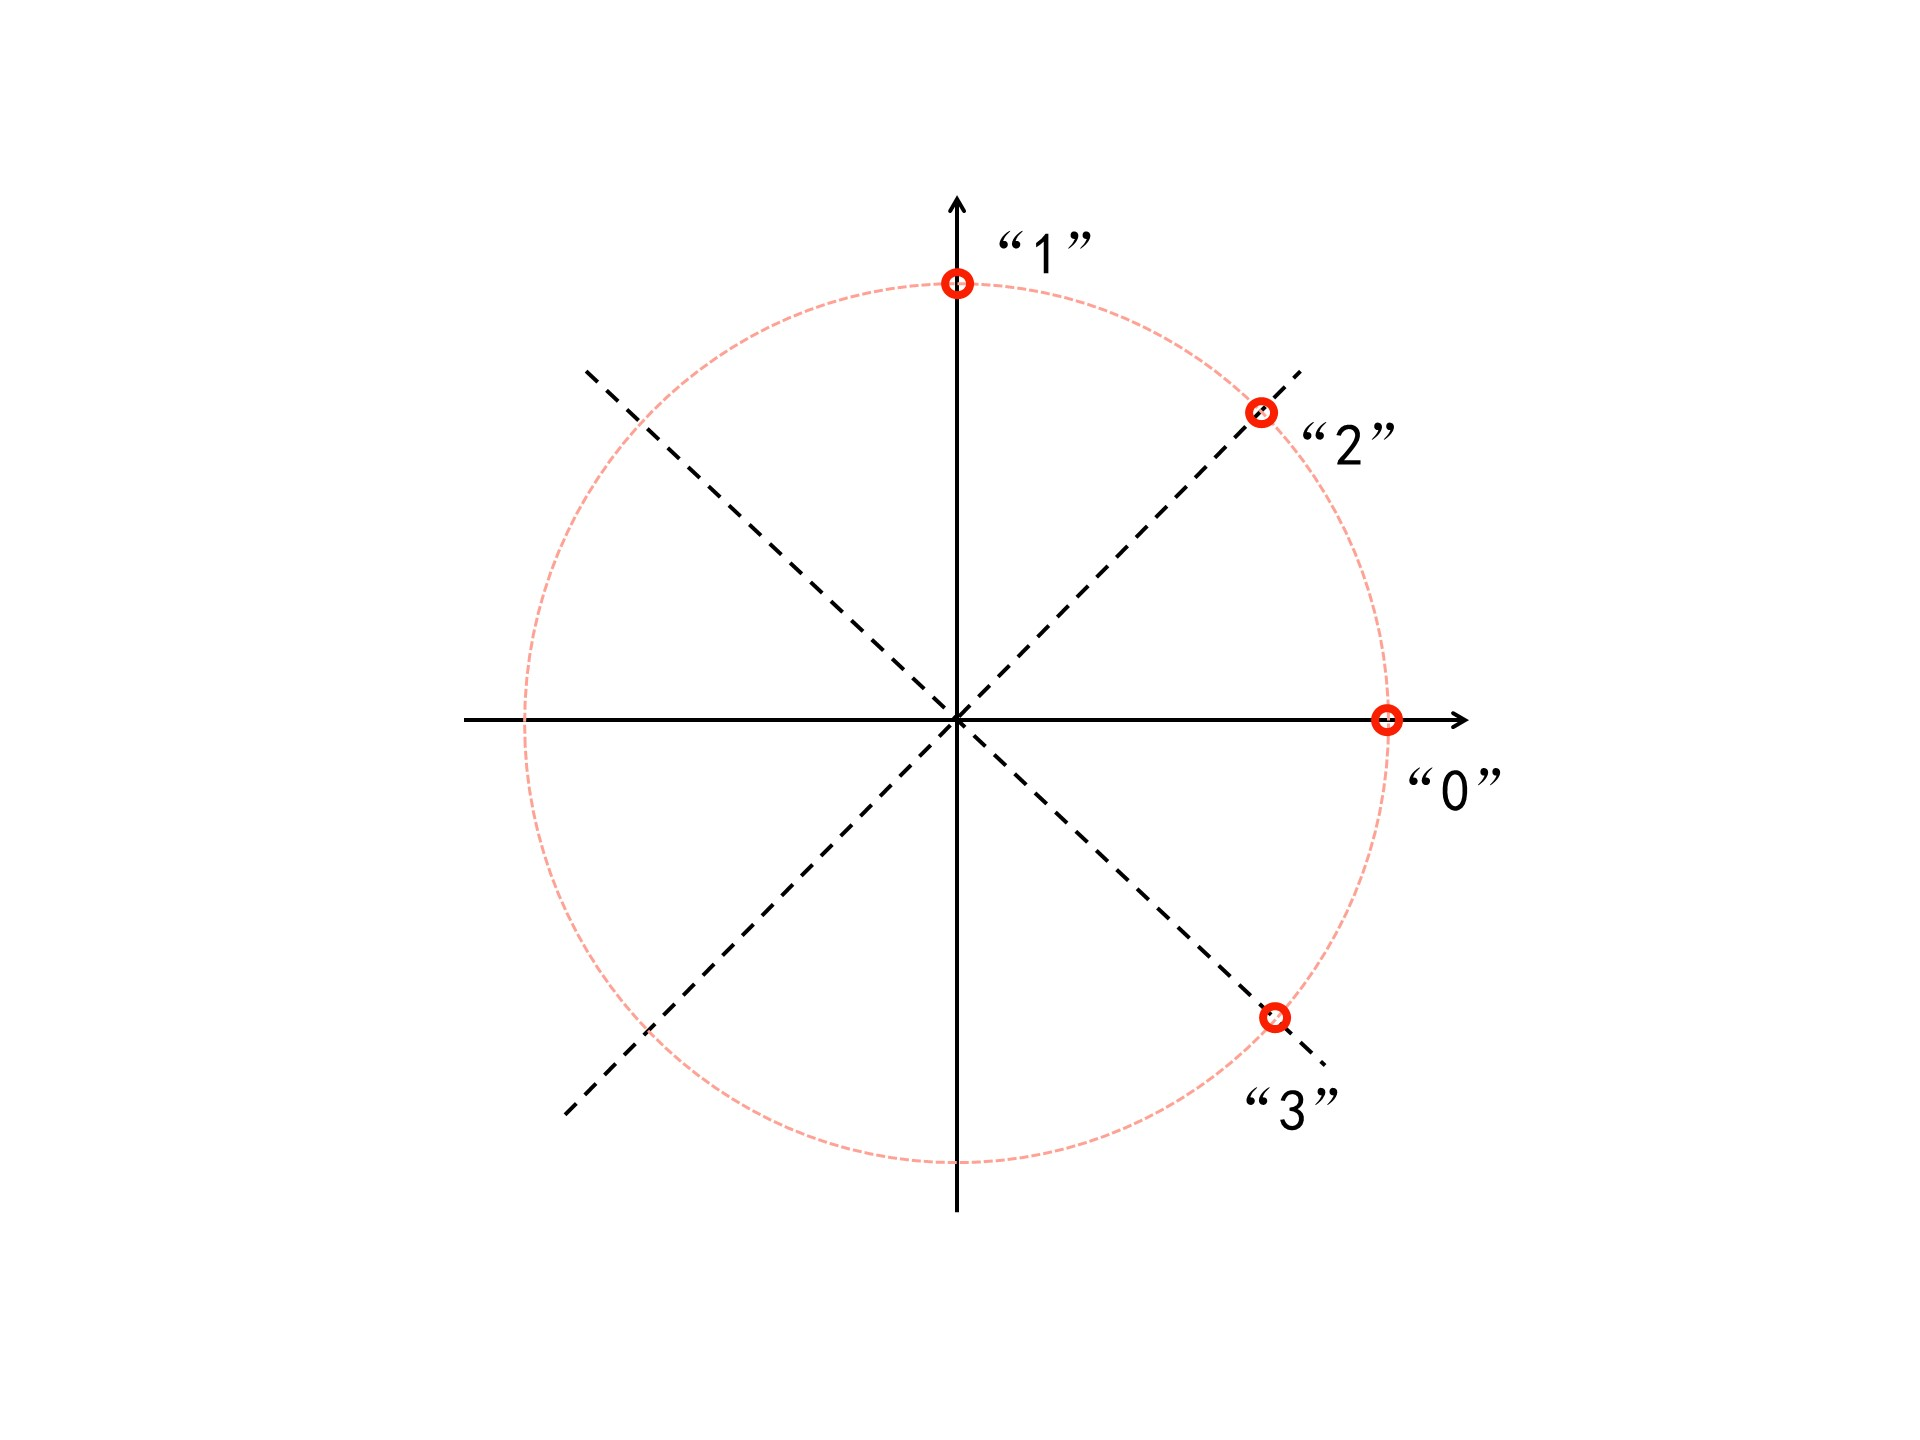
\includegraphics[width=6cm]{pic/qqpsk.jpg}
\caption{Constenlation diagram of quantum $\theta$ shift keying}
\label{qQPSK}
\end{figure}

The $\keta{+}$ wave is a superposition wave of the $\keta{0}$ and $\keta{1}$ waves and is best used as the input wave for parallel processing.
\begin{figure}[ht]
\begin{quantikz}
    \lstick{\ket{0}} & \gate{H} & \qw \rstick{\ket{+}}
\end{quantikz}
\caption{Use H gate to produce $\keta{+}$ wave.}
\label{H+}
\end{figure}

The $\keta{-}$ wave is also a superposition wave of the $\keta{0}$ and $\keta{1}$ waves, but is mostly used as the input wave phase kickback algorithm, which will be described in the following chapter.
\begin{figure}[ht]
\begin{quantikz}
    \lstick{\ket{0}} & \gate{X} & \gate{H} & \qw \rstick{\ket{-}}
\end{quantikz}
\caption{Use H gate to produce $\keta{-}$ wave.}
\label{H-}
\end{figure}

\section{Quantum gates for information processing}
Qubits are memory devices or communication channels. Quantum gates are processing devices that can change the modulation of $\theta$ and phase $\varphi$. As desired by the algorithms, the gates are concatenated or connected into circuits. Amplitude or the number of qubits is never changed until demodulation when qubits are measured. Measurements absorb the energy of qubits to extract digital data from them.

In the ket notation developed by physicists, a qubit gate operation is a quantum operator and can be noted by a letter $G$. In vector notation, a gate process can always be represented by a matrix. For example,
\begin{equation}
    \begin{pmatrix}
    cos\theta & e^{i\varphi} sin\theta \\
    e^{-i\varphi} sin\theta & cos\theta
    \end{pmatrix}
\end{equation}
which is unitary.
A algorithm or protocol is always depicted by a circuit diagram or series of matrix calculations. In circuit diagram, a qubit is shown as a line, and a gate as a rectangle.

\section{Hadamard gate}
Hadamard gate rotates the polarization $\theta$ of a qubit by 45 degrees. Its circuit symbol is letter "H" enclosed in a square. Rotating a $\keta{0}$ qubit 45 degrees obvious becomes a qubit of 45 degree polarization.
\begin{figure}[ht]
\begin{quantikz}
    \qw & \gate{H} &\qw
\end{quantikz}
\caption{Hadamard gate}
\label{Hadamard}
\end{figure}

\section{Pauli X, Y and Z gates}
A Z rotates a qubit's phase $\varphi$ by $180^{\circ}$ or $\pi$. A X gate exchanges $\keta{0}$ and $\keta{1}$. A Y gate exchanges $\keta{0}$ and $\keta{1}$ with additional phase change. They are best expressed in the vector notation as the Pauli matrices:
\begin{equation}
\begin{array}{rl}
    \sigma_1 & = \sigma_x = \begin{pmatrix}
        0 & 1 \\
        1 & 0
    \end{pmatrix} \\
    \sigma_2 & = \sigma_y = \begin{pmatrix}
        0 & -i \\
        i & 0
    \end{pmatrix} \\
    \sigma_3 & = \sigma_z = \begin{pmatrix}
        1 & 0 \\
        0 & -1
    \end{pmatrix}
\end{array}
\end{equation}

\chapter{Quantum communication protocols}

\section{BB84 protocol}
Encryption is used in everyday Internet communication. Encryption conceals the credit card numbers and passwords, which we send to the websites, from hackers or adversaries, who can eavesdrop the communication channels. Charles Bennett and Gilles Brassard proposed in 1984 a quantum encryption protocol\cite{BB84}. Named after the authors as the BB84 protocol, it secures communication from eavesdropping over the classical one-time-pad (OTP) encryption protocol\cite{Schneier} by taking advantage of the fact that a qubit cannot be divided for wire-tapping. Let's first describe how BB84 encrypts data as a version of the classical OTP protocol before describing how anti-eavesdropping protocol is added.

\subsection{BB84 as an encryption protocol}
By tradition, all communication encryption protocol is narrated as the scenario that Alice wants to transmit a series of data bits to Bob but fears Eve may eavesdrop the communication channel\cite{Schneier}. The encryption portion of the protocol goes like
- Alice has a second series of random bits of equal length to the data bits, which is the encryption key.
- Depending on the value of the key bit, 0 or 1, the transmitted data qubit uses either the $0\circ$ or $45\circ$ modulation base.
- Bob has the same series of key bits, and uses either the $0\circ$ or $45\circ$ modulation base to measure the received qubit.

%\begin{comment}[ht]
%\begin{tikzpicture}
 %   \path (-5, 0) node[anchor=east] (start) {$\keta{0}$}
 %   (-5,-2) node[Gate] (data) {Data bits}
 %   (-5,2) node[Gate] (key) {Key bits}
  %  (-4,0) node[Gate](dataCoder) {I/Z}
   % (-2,0% node[Gate](keyCoder) {I/H}
%    (2,0)%%% node[Gate] (keyDecoder) {I/H}
%    (4,0)%% node[Gate] (meter) {$\nearrow$}
%    (4,2)%% node[Gate] (keyD) {D-key bits} (keyDecoder)
%    (5,0)%% node[anchor=west] (output) {output};
%    \draw%% (start) -- (dataCoder) -- (keyCoder) -- (keyDecoder) -- (meter) -- (output);
%    \draw%[->] (data.east) -| (dataCoder.south);
%    \draw%[->] (key.east) -| (keyCoder.north);
%    \draw[->] (keyD.west) -| (keyDecoder.north);
%\end{tikzpicture}
%\caption{BB84 circuit}
%\label{BB84}
%\end{comment}

\begin{figure}[ht]
\begin{quantikz} %[wire types={q,c}]
    \lstick{Alice' data bits}  & \cwbend{1} \\
    \lstick{\ket{0}} & \gate{X} & \gate{H} &\qw & \gate{H} & \meter{} &\cw \rstick{data output} \\
    \lstick{Alice' key bits}  & \cw & \cwbend{-1} & & \cwbend{-1} & \cw \rstick{Bob's key bits}
\end{quantikz}
\caption{BB84 circuit}
\label{BB84}
\end{figure}

\subsection{Performance}
Channels: one.
Input Processing:
Output processing:
Transmission rate: one bit per qubit duty cycle.

\subsection{Adding authentication to BB84 protocol}
A quantum protocol such as BB84 is immune to wire-tapping, but like other protocols, it is vulnerable to attacks if Eve intercepts the qubits from Alice and send Bob qubits produced by herself. Not part of the BB84 protocol, the standard approach to detect such attacks is to add $m$ authentication bits, which are bits known to both Alice and Bob in advance, to every $n$ data bits:$a_1 a_2 ... a_m d_1 d_2 ...d_n$. If Bob finds the authentication bits not what he expects, he suspects the block's authenticity discards it.

\subsection{Key distribution}
All OTP protocols such as BB84 are theoretically beautiful but are not practical because they require encryption keys to be equal lengths as the data messages. It is a chicken and egg dilemma: how does Alice shares or distributes the series of secret key bits to Bob at the first place? Conventional public key exchange protocols are the current solutions. But they have many problems. They require expansive computation and may be broken by the power of quantum computing.

BB84 protocol and the quantum protocols following it do not depend on expansive computation. They recognize the fact that keys are random numbers. And key distribution or sharing can afford to lose some candidate key bits and does not require all candidate key bits being accepted by Bob. Alice can distribute all the candidate key bits to Bob. And Bob and Alice only need to agree on which of the candidate bits are "good" to use.

BB84 modifies the above protocol for key distribution in the following way:
- Alice generates two blocks of random bits of equal length with one block being the data bits -- or candidate key bits -- and another as the "encryption" key bits.
- Alice pairs the bits 00, 01, 10, or 11, and send it to Bob in the quantum channel (the qubit) mapped to the modulation points shown \ref{qQPSK}. Anyone who measures the qubit and gets a result of "0" cannot distinguish the actual code point is "00" or "10". So the original data is encrypted.
- Bob does not have the "encryption" key bits that Alice uses but has a series of key bits out of his random generation. And Bob demodulates each received qubit using his key bit and obtain his data bits.
- Alice and Bob then use a conventional communication channel to compare their corresponding key bits. If they agree, Alice and Bob keeps the candidate data bit. Otherwise, the candidate bit is discarded.

With many of the original data bits from Alice being discarded, what is good of BB84? The good part is that the kept data bits can be used as the key for future encryption. Therefore, BB84 is considered a quantum key distribution protocol. The quantum channel guarantees that it cannot be tapped. But it cannot prevent an eavesdropper Eve from intercepting the qubits in the channel. Eve may intercept the qubits without sending anything to Bob and may also attempt to reproduce the qubit to send to Bob. Because of the no-cloning theorem, Eve cannot reproduce the qubit to disguise the interception. So, key distribution with BB84 guarantees keys' confidentiality and integrity although the rate of key transmission may suffer from interception.

\section{2-qubit operations}
In conventional computers, 8, 16 or 32 bits are joined together to a unit of one byte, word or UINT32. Quantum circuits have their ways to join qubits into new units. If we look into 2 waveguide qubits, we see 4 waveguides, which we can label as $V_0$, $V_1$, $W_0$ and $W_1$. If we join the first two, we can make a superposition wave $a\keta[V]{0}+b\keta[V]{1}$ and allow only one quantum of wave in it. If we join the first and the third, physicists may call the new unit a joint wave while we keep the tradition of this book to call it a joint wave. Physicists note the new unit as $\keta[V]{0} \keta[W]{0}$ or simply $\keta{0}\keta{0}$. For quantum computing and communication, we allow two quanta in the joint wave.

\section{Control gates}
Assume $f(x)$ is a binary function mapping $x \in {0,1}$ to ${0,1}$. The control-f gate takes input waves $\keta{x}\keta{y}$, where $x$ and $y$ are either 0 or 1, and produce the output waves as shown below.
\begin{figure}[ht]
\begin{quantikz}
    \lstick{\ket{x}}  & \ctrl{1}  & \qw \rstick{\ket{x}} \\
    \lstick{\ket{y}} & \gate{f} &\qw \rstick{\ket{y\bigoplus f(x)}}
\end{quantikz}
\caption{Control-f gate}
\label{c-f}
\end{figure}
A particularly important type of control gates is the control-NOT or C-NOT gates, in which the $f$ is the Pauli $X$. A C-NOT gate is best described in vector notation as matrix
\begin{equation}
    \begin{pmatrix}
1 & 0 & 0 &0 \\
0 & 1 & 0 &0 \\
0 & 0 & 0 & 1 \\
0 & 0 & 1 & 0
\end{pmatrix}
\end{equation}

\section{Mostly used modulation points}
\subsection{The measurable points}
From 4 orthogonal waves, we have 4 joint waves $\keta{0}\keta{0}$, $\keta{0}\keta{1}$, $\keta{1}\keta{0}$ and $\keta{1}\keta{1}$, which are also orthogonal waves. We can use them as the base waves to represent 2-bit binary numbers 00, 01, 10 and 11. It's impossible to draw any 4-dimensional object using the 4 orthogonal base waves. But the constellation of QAM modulation diagram in Fig. \ref{QAM} shows to some extend the phase relation among the base waves except that two pairs of the waves in QPSK are 180-degree different in phase instead of orthogonal.

%\begin{figure}[ht]
%\begin{tikzpicture}
%    \draw[->] (-3.5,0) -- (3.5, 0);
 %   \draw[->] (0,-3.5) -- (0,3.5);
  %  \draw[dotted, red] (0,0) circle(3cm);
  %  \draw[red, fill] (2,0) circle(0.05cm) node[below right] {0};
   % \draw[red, fill] (0,2) circle(0.05cm) node[above right] {1};
    %\draw[red, fill] (3,0) circle(0.05cm) node[below right] {10};
%    \draw[red, fill] (0,3) circle(0.05cm) node[above right] {11};
%\end{tikzpicture}
%\caption{Constellation diagrams of two qubits}
%\label{QAM}
%\end{figure}

\subsection{Bell states}
Like in the cases of one qubit and QPSK, we can also use superpositions of the above base waves to come up with a new set of base waves:
\begin{equation}
\begin{array}{rl}
    \keta{\Phi^{+}} =& \frac 1 {\sqrt 2}| (\keta{0}\keta{0}+\keta{1}\keta{1}),\\
    \keta{\Phi^{-}} =& \frac 1 {\sqrt 2}| (\keta{0}\keta{0}-\keta{1}\keta{1}),\\
    \keta{\Psi^{+}} =& \frac 1 {\sqrt 2}| (\keta{0}\keta{1}+\keta{1}\keta{0}),\\
    \keta{\Psi^{-}} =& \frac 1 {\sqrt 2}| (\keta{0}\keta{1}-\keta{1}\keta{0}).
\end{array}
\end{equation}
The second set of base waves can be considered 45 degree rotated from the first set. Physicists call them Bell state waves and use the funny symbols to note them. They are in the form $cos\theta |b_i> + sin\theta |b_j>$. They are no longer separable waves.

We can use 8 waves from the 2 sets of bases to represent numbers of 3 bits as shown in Fig. \ref{8QAM}.

\section{Design patterns}

\subsection{Producing Bell states}
\begin{figure}[ht]
\begin{quantikz}
    \lstick{\ket{+}}  & \ctrl{1} & \qw \rstick[2]{\ket{\Phi^+}} \\
    \lstick{\ket{0}} & \gate{X} &\qw 
\end{quantikz}
\caption{Producing Bell states}
\label{BS}
\end{figure}
Changing the input waves from $\keta{+}$ to $\keta{-}$ or from $\keta{0}$ to $\keta{1}$, we can obtain the other Bell states.

\section{Superdense coding}
Superdense coding is also called dense coding. With the consideration of two qubits as one wave, modulation of one qubit is modulating the shared $\theta$ of the entanged wave. The modulation appears to be upon one qubit. But the information is actually coded into two qubits.

The operation first creates entanglement $\keta{\Phi^{+}}$.

\begin{table}[]
\caption{Modulate one qubit twice to encode 2 bits}
\label{DenseCodingTable}
\begin{tabular}{lll}
Digital input & Modulating operation & gate                 \\
00 & None   & None \\
01 & $90 degree$& Z gate \\
10 & Mirror switch $\keta{0}$ and $\keta{1} $ &X gate \\
11 & Mirror switch $\keta{0}$ and $\keta{1}$ and $90 degree$ &X gate
\end{tabular}
\end{table}

\subsection{Circuit diagram}
\begin{figure}[ht]
\begin{quantikz}%[slice all, slice style={shorten <=8mm}, slice label style = {yshift=-38mm} ]
    & & &\lstick{Alice' 2nd bit}  & \cwbend{2} \\
    & & \lstick{1st bit}  & \cwbend{1} \\
    \lstick{\ket{0}} & \gate{H} &\ctrl{1} & \gate{Z} & \gate{X} &\ctrl{1} & \gate{H} & \meter{} &\cw \rstick{Bob's 1st bit} \\
    \lstick{\ket{0}} & \qw      & \targ{} \slice[style={shorten <=12mm}, label style={yshift=-38mm}]{1} & \qw \slice[style={shorten <=12mm}, label style={yshift=-38mm}]{2} & \qw \slice[style={shorten <=12mm}, label style={yshift=-38mm}]{3} & \targ{} & \qw & \meter{} & \cw \rstick{Bob's 2nd bit}
\end{quantikz}
\caption{Superdense coding circuit}
\label{DenseCoding}
\end{figure}

\section{Teleportation}
\subsection{Circuit diagram}
\begin{figure}[ht]
\begin{quantikz}%[slice all, slice style={shorten <=8mm}, slice label style = {yshift=-38mm} ]
    & & \lstick{Alice' wave a\ket{0}+b\ket{1}}  & \ctrl{1} & \gate{H} & \meter{} &\cw \rstick{Alice' 1st bit} \\
    \lstick{\ket{0}} & \gate{H} &\ctrl{1} & \targ{} & \qw& \meter{} &\cw \rstick{Alice' 2nd bit} \\
    \lstick{\ket{0}} & \qw      & \targ{} \slice[style={shorten <=2mm}, label style={yshift=-38mm}]{1} & \qw & \qw & \qw \rstick{Bob's wave}
\end{quantikz}
\caption{Teleportation circuit}
\label{Teleportation}
\end{figure}

Similar to dense coding, quantum teleportation is to modulate an analog signal to one qubit of a $|BS1>$ two-qubit wave. The analog signal comes in the form of a qubit, which we call it the signal qubit. And the wave may be written as $a \keta{0} + b\keta{1}$.
\begin{equation}\label{}
\begin{array}{rl}
    & (a \keta{0} + b\keta{1}) \frac 1 {\sqrt 2}(\keta{0}\keta{0}+\keta{1}\keta{1}) \\
    = & \frac 1 {\sqrt 2}| (\keta{0}\keta{0}+\keta{1}\keta{1}) (a \keta{0} + b\keta{1}) \\
    +& \frac 1 {\sqrt 2}| (\keta{0}\keta{0}-\keta{1}\keta{1}) (a \keta{0} - b\keta{1}) \\
    +& \frac 1 {\sqrt 2}| (\keta{0}\keta{1}+\keta{1}\keta{0}) (a \keta{0} + b\keta{1}) \\
    +& \frac 1 {\sqrt 2}| (\keta{0}\keta{1}-\keta{1}\keta{0}) (a \keta{0} - b\keta{1})
\end{array}
\end{equation}

\begin{table}[]
\caption{Modulate one qubit to encode 2 bits}
\label{TeleportationTable}
\begin{tabular}{lr}
Alice's output $d_1 d_0$ & Bob's qubit  \\
00 & $a\keta{0}+b\keta{1}$ \\
01 & $a\keta{1}+b\keta{0}$ \\
10 & $a\keta{0}-b\keta{1}$  \\
11 & $a\keta{1}-b\keta{0}$ 
\end{tabular}
\end{table}

Alice has a qubit with information S and shares a pair of qubits with Bob. The pair is one of the 4 known eigenwaves and has 2 bits of information. The total input information is therefore S+2. At the output, Alice measures the first 2 qubits against the same 4 eigenwaves and tells Bob the result, which has 2 bits of information. If no information is lost, the information in the 3rd qubit should be S.

\section{Quantum secure direct communication (QSDC)}
QSDC is an adaptation of quantum teleportation to key distribution. The key transmission rate is 1 bit per qubit duty cycle and is a much improvement over the BB84 protocol.

\chapter{Deutsch's and related algorithms}

\section{Deutsch's algorithm}
A one-bit function $f$ mapping \{0,1\} -\> \{0,1\} can have 4 possible outputs, which are 2 bits of information. But the outputs belong to 2 categories, constant or balanced, which are an 1-bit information as of $f(1)+f(0)$. We can't obtain the 2-bit information using one operation but can obtain the 1-bit information if we feed the function with the $\keta{+}$ qubit:
\begin{equation}\label{DeutschF1}
\begin{array}{rl}
    U_f(\frac 1 {\sqrt 2} (\keta{0}+\keta{1}) ) = & \frac 1 {\sqrt 2} (e^{2\pi i f(0)} \keta{0}+ e^{2\pi i f(1)} \keta{1}) \\
    = & \frac 1 {\sqrt 2} e^{2\pi i f(0)} (\keta{0}+ e^{2\pi i [f(1)-f(0)]} \keta{1})
\end{array}
\end{equation}

From above derivation, we see that it takes one operation of the $F$ gate to evaluate both $f(0)$ and $f(1)$. But the result still requires two measurements, one to determine $f(0)$ and the other to determine $f(1)-f(0)$. For two measurements, we need the help of another qubits.

\subsection{Phase kick back}
\begin{figure}[ht]
\begin{quantikz}
    \lstick{\ket{x=0/1}}  & \ctrl{1} & \qw \rstick{$(-1)^{f(x=0/1)}$ \ket{x=0/1}} \\
    \lstick{\ket{-}} & \gate{f} &\qw \rstick{\ket{-}} 
\end{quantikz}
\caption{Producing Bell states}
\label{phaseKick}
\end{figure}

With the help of a C-NOT gate, the 2 bits of information modulated in one qubit can be transfered to two qubits and therefore can be all extracted.

\subsection{Circuit diagram}
\begin{figure}[ht]
\begin{quantikz}[scale=1.3]
    \lstick{\ket{0}} & \gate{H} & \ctrl{1} \slice{$(-1)^{f(0)}$\ket{0}+$(-1)^{f(1)}$ \ket{1} }  & \gate{H} & \meter{} &\cw \rstick{$f(1)-f(0)$} \\
    \lstick{\ket{1}} & \gate{H} & \gate{f} &\qw \rstick{\ket{-}}
\end{quantikz}
\caption{Deutsch's algorithm circuit}
\label{Deutsch}
\end{figure}

\subsection{Performance}
Processing: two quantum gates - one operation per gate; one measurement.
Memory: one qubit for the processing. But for output, two qubits are required.


\section{Mostly used modulation points}
\subsection{Measurement bases}
The measurement base waves are $\keta{x_0}\keta{x_1}\keta{x_2} ...\keta{x_{n-1}}=\prod^{n-1}_{i=0}$, where $x_i in \{0, 1\}$.

\subsection{Evenly mixed wave and Fourier bases}
Expanding on the idea of the $\keta{+}$ wave in \ref{Sec-Plus}, we can have a wave
\begin{equation}
\begin{array}{rl}
    \keta{s_0} &= \frac 1 {\sqrt{2}} (\keta[0]{0}+\keta[0]{1}) \frac 1 {\sqrt{2}} (\keta[1]{0}+\keta[1]{1})
    ... \frac 1 {\sqrt{2}} (\keta[n-1]{0}+\keta[n-1]{1}) \\
    &= \frac 1 {2^{n/2}} (\keta{b_0}+\keta{b_1}+...+\keta{b_{N-1}})
 \end{array}
\end{equation}
which is an evenly mixture of the $n$-qubit bases. But what are the orthogonal waves similar to the $\keta{-}$ of one qubit?
\begin{equation}
\begin{array}{rl}
\keta{s_k} &= \frac 1 {\sqrt{2}} ({\keta{0}}_0+{\keta{1}}_0)
    \frac 1 {\sqrt{2}} ({\keta{0}}_1+e^{\frac {k*2 \pi i} 2}{\keta{1}}_1)
    ...  \frac 1 {\sqrt{2}} ({\keta{0}}_{n-1}+e^{\frac {(n-1)*2\pi i} 2^(n-1)}{\keta{1}}_{n-1}) \\
    ... \\
    &= \frac 1 {\sqrt{N}} \prod^{n-1}_{l=0} ({\keta{0}}_l+e^{\frac {k\times l \times 2\pi i} 2^l}{\keta{1}}_l) where k=0, 1, ...N-1.
\end{array}
\end{equation}
Like the $\keta{+}$ and $\keta{-}$ waves, each of the $\{\keta{s_k}, k=0, 1, ... N-1\}$ waves is a mixture of all the base waves, but they have different orientations in the $N$ dimension Hilbert space.

\section{Design patterns}

\subsection{Producing equal superposition}

\subsection{Quantum Fourier transform}
Classical discrete Fourier transform maps a set of $N$ complex numbers ${x_0, x_1, ..., x_{N-1}}$ to another $N$ complex numbers
\begin{equation}
    y_k = \frac 1 {\sqrt{N}} \sum^{N-1}_{n=0} x_n\omega_{N}^{-nk}, k = 0, 1, 2, ..., N-1,
\end{equation}
where $w_N = e^{\frac {2\pi i} N }$. For physicists and engineers, the numbers ${y_n}$ help to reflect prominently the periodic patterns such as their frequency in $x_n$. For the same purpose, quantum Fourier transform is defined mathematically as follow but is easier to be realized by quantum gates:
\begin{equation}
    y_k = \frac 1 {\sqrt{N}} \sum^{N-1}_{n=0} x_n\omega_{N}^{xk}, k = 0, 1, 2, ..., N-1,
\end{equation}
where $x = x_0 + x_1 2^1 + x_2 2^2 + ... +x_{N-1} 2^{N-1}$. In vector notation, $F_N$ is a unitary matrix, and its $i, j$ element is
\begin{equation}
    f_{i,j} = \omega^{i.j}.
\end{equation}
This matrix is the same matrix as for the discrete Fourier transform. Therefore, quantum Fourier transform is equivalent to discrete Fourier transform.

\subsubsection{Complexity}

\subsection{Phase estimation}
\subsubsection{Complexity}

\section{Grover's algorithm}
Like the Deutsch's algorithm, the Grover's algorithm also assumes a blackbox function $f(x)$ whose variable $x$ is a $n$-bit binary variable. Its result is a single-bit value and is always 1 except for a few unknown $x=x_w$ at which $f(x_w)=-1$. The goal of the algorithm is to find the $x_w$. Lov Grover proposed in 1996 that quantum computer can solve it faster than conventional computers.

Let's assume there is one and only one solution $x_w$ as an example, and note $x_w$ as $w_{n-1}...w_i...w_1 w_0$ in binary where $w_i = 0 or 1$, and $\Vec{w} = (0, 0, ..., 1 at i=w, ..., 0)^T$ as a $2^n-1$ dimensional vector. Using classical computers, we'd feed each of the $2^n -1$ possible numbers of $x_w$ at a time to $f$ to test whether the result equals $-1$. The worst case is that we have to do $2^n-1$ evaluations of $f(x)$ to find out $x_w$. We of course wish to explore all the possible $x_w$ at the same time. We naturally choose $\vec{S} = \frac 1 {\sqrt{2^n}} (1, 1, ...1)^T$, which is the sum of all the bases of the qubits, to feed the oracle function $f$.

We know, $\vec{S} = \vec{S} - \frac 1 {\sqrt{2^n}} \vec{w}) + \frac 1  {\sqrt{2^n}} \vec{w}$. Apparently, $\vec{S_1}  = \vec{S} - \frac 1 {\sqrt{2^n}} \vec{w}$ is a vector orthogonal to $\vec{w}$, and applying the $F$ gate to it does not change its phase. Therefore, $F(\vec{S}) = F(\vec{S_1}) + F(\frac 1  {\sqrt{2^n}} \vec{w})  = \vec{S_1} - \frac 1 {\sqrt{2^n}} \vec{w}$. We see that 
\begin{itemize}
    \item applying the $F$ gate turns vector $\vec{S}$ toward $-\vec{w}$
    \item applying the $F$ gate to $\vec{S_1}$ makes no change.
\end{itemize}
Therefore, can we apply $F$ gate $2^n$ times and turn $\vec{S}$ completely to $-\vec{w}$? But applying $F$ gate once more will change the phase of the $\vec{w}$ vector back. We need to change the sign of vector $\vec{w}$ first while preserving its angle with $\vec{S}$ before applying $F$ gate again. This can be accomplished by apply gate $U_S = 2 \vec{S}X\vec{S} -I$, which flip $\vec{w}$ around the vector $\vec{S}$. However, when implementing this flip, we need to rotate $vec{S}$ to the $\vec{0}$, do the flip, and rotate the frame back to $\vec{S}$.

\begin{figure}[ht]
\begin{tikzpicture}
\coordinate (S) at (30:3);
    \draw[red, fill] (S) circle(0.05cm)  node[right] {$\vec{S}$};
    \draw[->, dashed] (0,0) -- (S);
    \draw[->] (0,0) -- (3, 0) node[below] {$\vec{w_v}$};
    \draw[->] (0,0) -- (0,3) node[right] {$\vec{w}$};
    %\draw[dotted, red] (0,0) circle(3cm);
\end{tikzpicture}
\caption{Applying F gate}
\label{grover}
\end{figure}

\subsection{Complexity}

\section{Simon's algorithm}
The Simon's algorithm assumes a blackbox oracle function $f(x)$ whose variable $x$ is a $n$-bit binary variable. Its results are $m$-bit values that are periodic, but the period $t$ is unknown -- $f(x+t)=(fx)$ for all $x$. How do we find the period $t$? Of course, we are tempted to play the trick again of feeding $\vec{S} = \frac 1 {\sqrt{2^n}} (1, 1, ...1)^T$ to the oracle function $f$. We have
$f(\vec{S}) = \frac 1  {\sqrt{2^n}} \sum_x f(x)$.

\subsection{Circuit diagram}
\begin{figure}[ht]
\begin{quantikz}%[slice all, slice style={shorten <=8mm}, slice label style = {yshift=-38mm} ]
    & & &\lstick{Alice' 2nd bit}  & \cwbend{2} \\
    & & \lstick{1st bit}  & \cwbend{1} \\
    \lstick{\ket{0}} & \gate{H} &\ctrl{1} & \gate{Z} & \gate{X} &\ctrl{1} & \gate{H} & \meter{} &\cw \rstick{Bob's 1st bit} \\
    \lstick{\ket{0}} & \qw      & \targ{} \slice[style={shorten <=12mm}, label style={yshift=-38mm}]{BS1} & \qw \slice[style={shorten <=12mm}, label style={yshift=-38mm}]{BS2} & \qw \slice[style={shorten <=12mm}, label style={yshift=-38mm}]{BS3} & \targ{} & \qw & \meter{} & \cw \rstick{Bob's 2nd bit}
\end{quantikz}
\caption{Simon's algorithm}
\label{Simon}
\end{figure}

\subsection{Complexity}
Using conventional computer, finding the period takes $2^{n/2}$ operations.

\section{Shor's algorithm}
Much of modern day cryptography is based on the difficulty of factoring large integer numbers. Almost all Internet connections from our mobile phones and computers are based on AES, which is a private key encryption algorithm, and RSA or DH algorithms for key exchange.

For a positive integer $M$, how can we find out whether it has factors? A naive approach is to iterate over
$a=2, 3, ..., [M/2]$ one by one to see whether $M$ modulo $a$ is zero or $M mod a = 0$. Mathematicians have found a shortcut basing on the fact that if a pair of positive integers $a < N$ and $r$ exist, such that $a^r = 1(mod M)$, and that if they exist and $r$ is an even number, $(a^{r/2}+1)(a^{r/2}-1) = 0 (mod M)$. $r$ is called the order of $a$. The ranges of $a$ and $r$ are much smaller than $[M/2]$. But, beside some trivial solutions, iterating over all the possible $a$ and $r$ is still a daunting task. Peter Shor, in his 1997 monumental paper\cite{1997Shor}, described a quantum algorithm, which finds the existence of $r$ and its value without iteration for every given $a$.

With all the design patterns, which we have learned so far, how would we design such an algorithm? We may simply extend the ideas behind the Deutsch's algorithm to the $n$ dimension, where $n$ is the closest integer for $M < 2^n$.
1. feed the function $f(x) = a^x (Mod M)$ with the evenly mix quantum waves $\keta{s_0}$
2. use phase kickback to transfer the values of $f(j), j\in \{0,N-1\}$, which should have periodicity of $r$, to the phases of the waves in the Fourier base
3. use phase estimate to reveal the information containing $r$.

For phase kickback to work, we need to find an eigen-waves of $U_f$,
\begin{equation}\label{keta_u}
    \keta{u} = \sum^{r-1}_{j=0} c_j \keta{a^j (mod M)}.
\end{equation}
If we assume the eigen-values are $e^{2\pi i \frac k r}$ where $k=0, 1, 2, ..., r-1$. We derive the corresponding eigen-waves to be
\begin{equation}\label{keta_uk}
    \keta{u_k} = \frac 1 {\sqrt{r}} \sum^{r-1}_{j=0} e^{-{\frac {2\pi} r} kj} \keta{a^j (mod M)}
\end{equation}

However, we don't know the value of $r$ at the first place except the trivial $u_0$. How can we produce any of the non-trivial eigen waves to feed the operator $U_f$? Fortunately, the even mixture of the eigen waves
\begin{equation}\label{sum_u}
    \frac 1 {\sqrt{r}} \sum^{r-1}_{k=0}\keta{u_k} = \frac 1 r \sum^{r-1}_{k=0} \sum^{r-1}_{j=0} e^{-{\frac {2\pi} r} kj} \keta{a^j (mod M)} = \sum^{r-1}_{j=0} \delta_j,0 \keta{a^j (mod M)} = \keta{1}
\end{equation}
is a wave that we know how to produce. Feed it to the control-$U_f$ with $j$ being the control-variable value, we have
\begin{equation}\label{ctrl_u}
\begin{array}{rl}
 \sum^{N-1}_{j=0} \keta{j} \keta{1} \xrightarrow{U_{f(j)}} & \sum^{N-1}_{j=0} \keta{j} U_{f(j)} \frac 1 {\sqrt{r}} \sum^{r-1}_{k=0}\keta{u_k}\\
    = & \frac 1 {\sqrt{r}} \sum^{r-1}_{k=0} \sum^{N-1}_{j=0} \keta{j} e^{2\pi i \frac kj r} \keta{u_k}\\
    = & \frac 1 {\sqrt{r}} \sum^{r-1}_{k=0} \keta{s_{k/r}} \keta{u_k}
\end{array}
\end{equation}

\subsection{Circuit diagram}
\begin{figure}[ht]
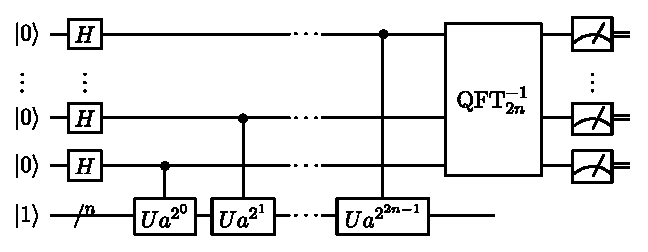
\includegraphics[width=12cm]{pic/Shor_algorithm.eps}
\caption{Circuit of Shor's algorithm}
\label{ShorAlgorithm}
\end{figure}

\subsection{Complexity}

\section{Boson sampling algorithms}

\subsection{Complexity}

\chapter{Noise, and error correction}
\section{Channel capacity}
According to Shannon theorem, under noise, the channel capacity is $C = 2B (1+SNR)$.


\chapter{Appendix: Qubit devices}\label{A-qubit}
\section{Types of waves by propagating characteristics}
Radio-frequency (RF) electromagnetic waves are used for mobile communications including Wi-Fi. They can spread to everywhere if not being blocked or confined by reflective matters. Light waves -- electromagnetic waves with wavelength ranging from sub-micron to a few microns -- are used for optical communications. They can be channeled by optical waveguides such as optical fibers to explore different paths. They are confined in two dimensions -- the lateral dimensions -- but propagate in the dimension along the axes of the waveguides or fibers. Communication, quantum or not, must use propagating waves, of course. With difficulties, propagating waves may also be used in quantum computing.

Without confinement, a wave can propagate through out space and time and does not have definite size or location. If an electromagnetic wave is confined in three dimensions, such as in a microwave oven, the wave cannot propagate anywhere other than being reflected back and forth within the confinement. And only standing waves of specific frequencies can exist. The allowed frequencies are discrete. Standing waves are good for storing information. Superconductor qubits are built by standing waves of electrons as we describe below. Standing waves may be best visualized and understood by the vibrations of a guitar string. When a string is plucked, the propagation of the vibrations are stopped and reflected by the two fixed ends. Only the waves whose phases coincide after a complete round trip of reflection survive while the other waves cancel each other and die off.

Another type of waves, which we may call trapped waves, are not confined by anything with boundaries but are trapped by forces extending to infinity. Electrons in an atom are trapped waves by the electric force of the nucleus' positive charges. The waves extend to infinity but are concentrated within a nanometer around the nucleus. Trapped waves are also good for storing information. Trapped-ion qubits are built by trapped electron waves.

\chapter{Appendix: Quantum gates}

\subsection{C-NOT gate}
\subsection{Phase kick back}

\subsection{Generator}
How a qubit is put in the wave of "0" or "1" depends on the specific implementation. A quantum circuit diagram is usually drawn with a qubit starts in the "0" or occasionally in the "1" wave.

\subsection{Hadamard gate}
To modulate a qubit in the 10 or 11 wave, a $\theta_pm = 45$ degree phase shifter in the constellation diagram is needed. In the Bloch sphere, a $\theta_q =90, \phi=0$ phase shift is needed. Such a phase shifter is called a Hadamard gate. In the ket notation, $|11> = 1 over [\sqrt 2] (\keta{0} + \keta{1})$ and $|10> = 1 over [\sqrt 2] (\keta{0} - \keta{1})$. So, as a vector transformation, the Hadamard gate is a transformation matrix:
\begin{equation}
    \frac 1 {\sqrt 2}
    \begin{pmatrix}
1 & 1 \\
1 & -1
\end{pmatrix}
\end{equation}


%\backmatter

\addcontentsline{toc}{chapter}{Bibliography}
\chapter*{Bibliography}
\bibliographystyle{unsrt}
   \bibliography{qcc}

\addcontentsline{toc}{chapter}{Index}
\printindex
\end{document}